\subsection{\efake background estimation}
\label{sec:background-estimation-efake}
Electrons are reconstructed from the EM calorimeter energy deposits and the associated track reconstructed in the inner detector. Where photons are reconstructed from the EM calorimeter energy deposits. The reconstruction of electrons and photons is similar, and the main difference is that the electron has a track associated with it. Therefore, it is possible that an electron is misidentified as a photon, which is called $e\to\gamma$ fake. It is an important background in the single-lepton channel. The main processes contributing to this background are the \ttbar dileptonic decays (\chee and \chemu channels) and $Z\to ee$ decay, where one electron fakes a photon. Although the same algorithm is used to reconstruct electrons and photons in MC and data, the MC simulation doesn't model the $e\to\gamma$ fake events correctly. This discrepancy in the $e\to\gamma$ fake rate between data and MC is corrected by using a fake rate scale factor, which is the ratio between fake rate in data and the fake rate in MC. The fake rate is defined in ~\cref{sec:egammafakes_fr}. To calculate fake rate in data and in MC, fake enriched control regions are defined using \zee process. If electron from \zee process is misidentified as a photon, then it will be a fake photon. Two control regions are defined, \zee and \zegamma. Since there is no \zegamma process in SM, in this control region the photon are expected to be fakes from electron from \zee process. The definition of these control regions is given in Section~\ref{sec:egammafakes_cr}.


Section \ref{sec:egammafakes_cr} defines the control regions used for the study. 
%, which are expected to be dominated by the $Z\to ee$ process. 
Section \ref{sec:egammafakes_source} describes the studies on the source of $e\to\gamma$ fakes by matching them to the truth level particles. Section \ref{sec:egammafakes_fr} defines the fake rate and contains the calculation of the fake rate scale factor.
%Section \ref{sec:egammafakes_closure} discusses the application of the fake rate scale factor and the closure of the method.

\subsection{Control regions}
\label{sec:egammafakes_cr}

To study the $e\to\gamma$ fake rate, a fake enriched control region is defined by selecting events having a pair of back-to-back electron and photon, which will be called $e\gamma$ control region. The requirements include:
\begin{itemize}
\item Exactly one electron which is trigger matched.
\item At least one photon. The leading \pt photon is referred simply as photon in the following.
\item The opening angle between the electron and the photon to be larger than 150 degrees. This requirement helps to reduce different backgrounds due to hadron being misreconstructed as photon and prompt photons radiated from the electron.
\item The invariant mass of the electron and the photon to be within 50 GeV around the $Z$ mass. 
\end{itemize}
In the selected events, the electron is called \textit{tag electron} and the photon is called \textit{probe photon}.

Another control region, that will be called $ee$ control region, is defined in exactly the same way as above, but by replacing the photon in the requirements with an electron which should have opposite charge sign with respect to the tag electron. Thus, this electron is called \textit{probe electron} and is used as a reference to be compared with the probe photon to define the fake rate later. Complete definition of the $ee$ and $e\gamma$ control regions is shown in the Figure~\ref{fig:egammafake_cr}.

\begin{figure}[!htbp]
\centering
%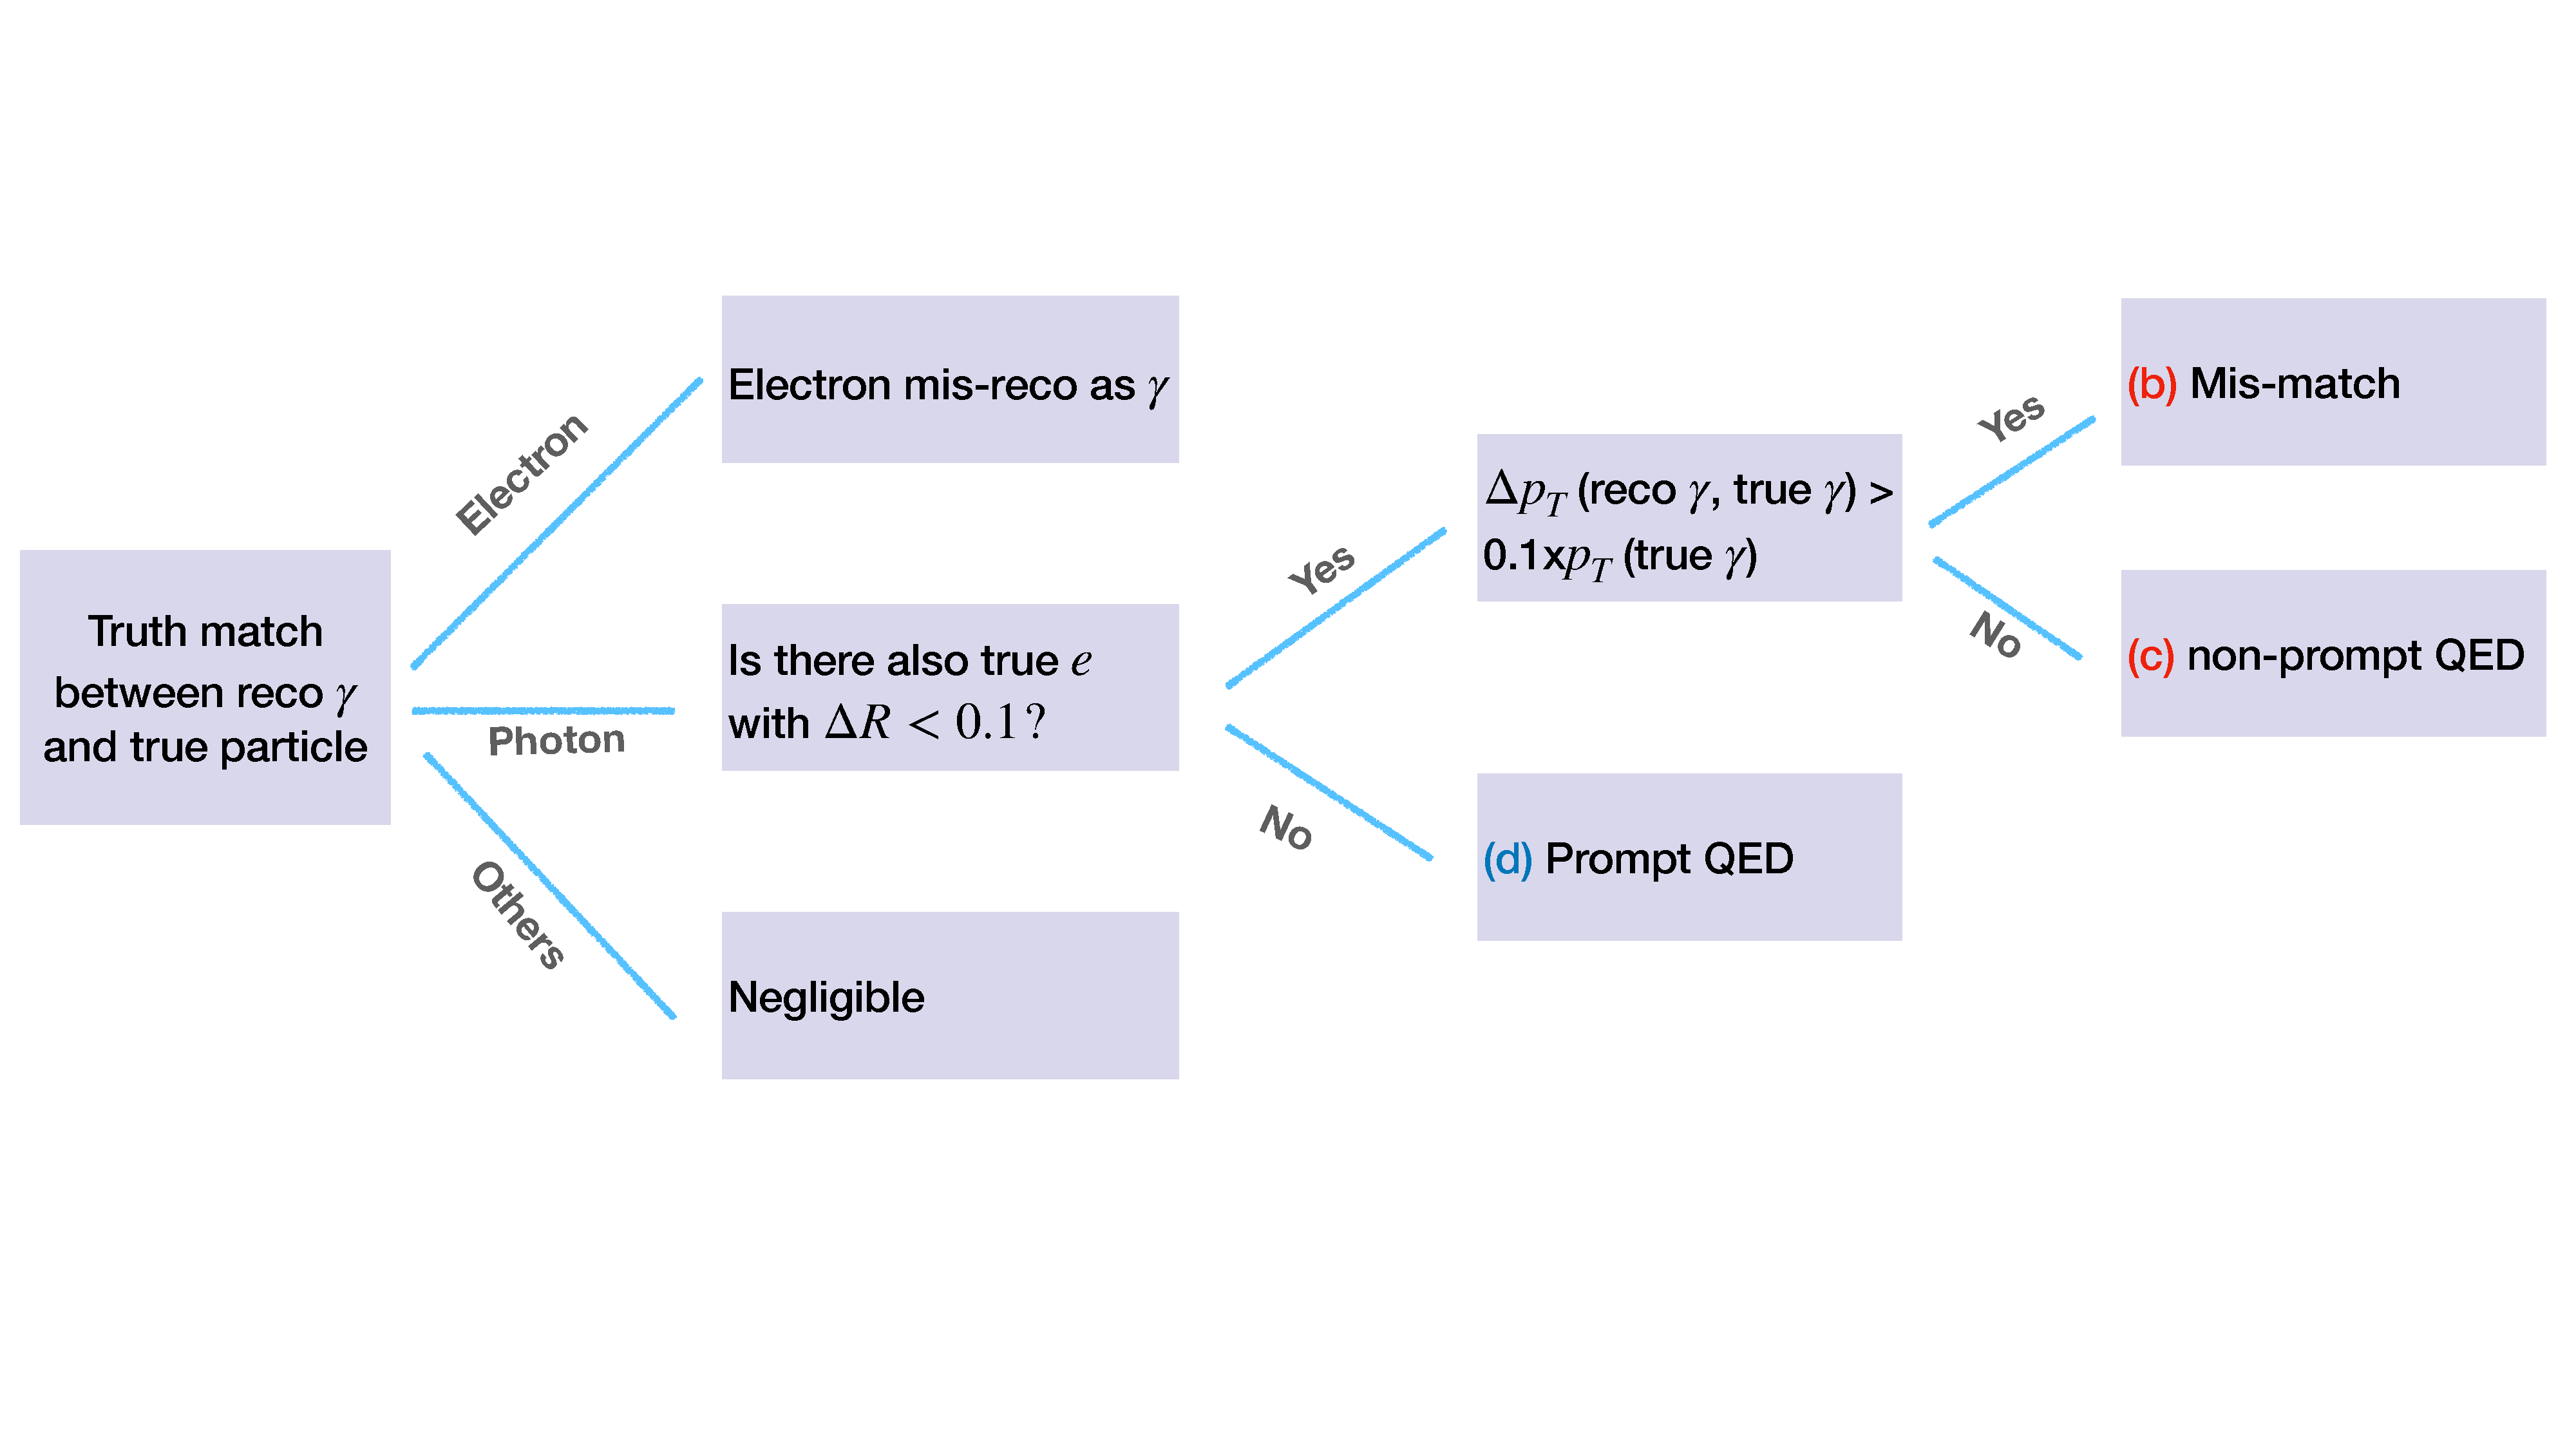
\includegraphics[width=0.49, scale=2.0\textwidth]{figures/egammafakes/efake_truth_matching.pdf}}
{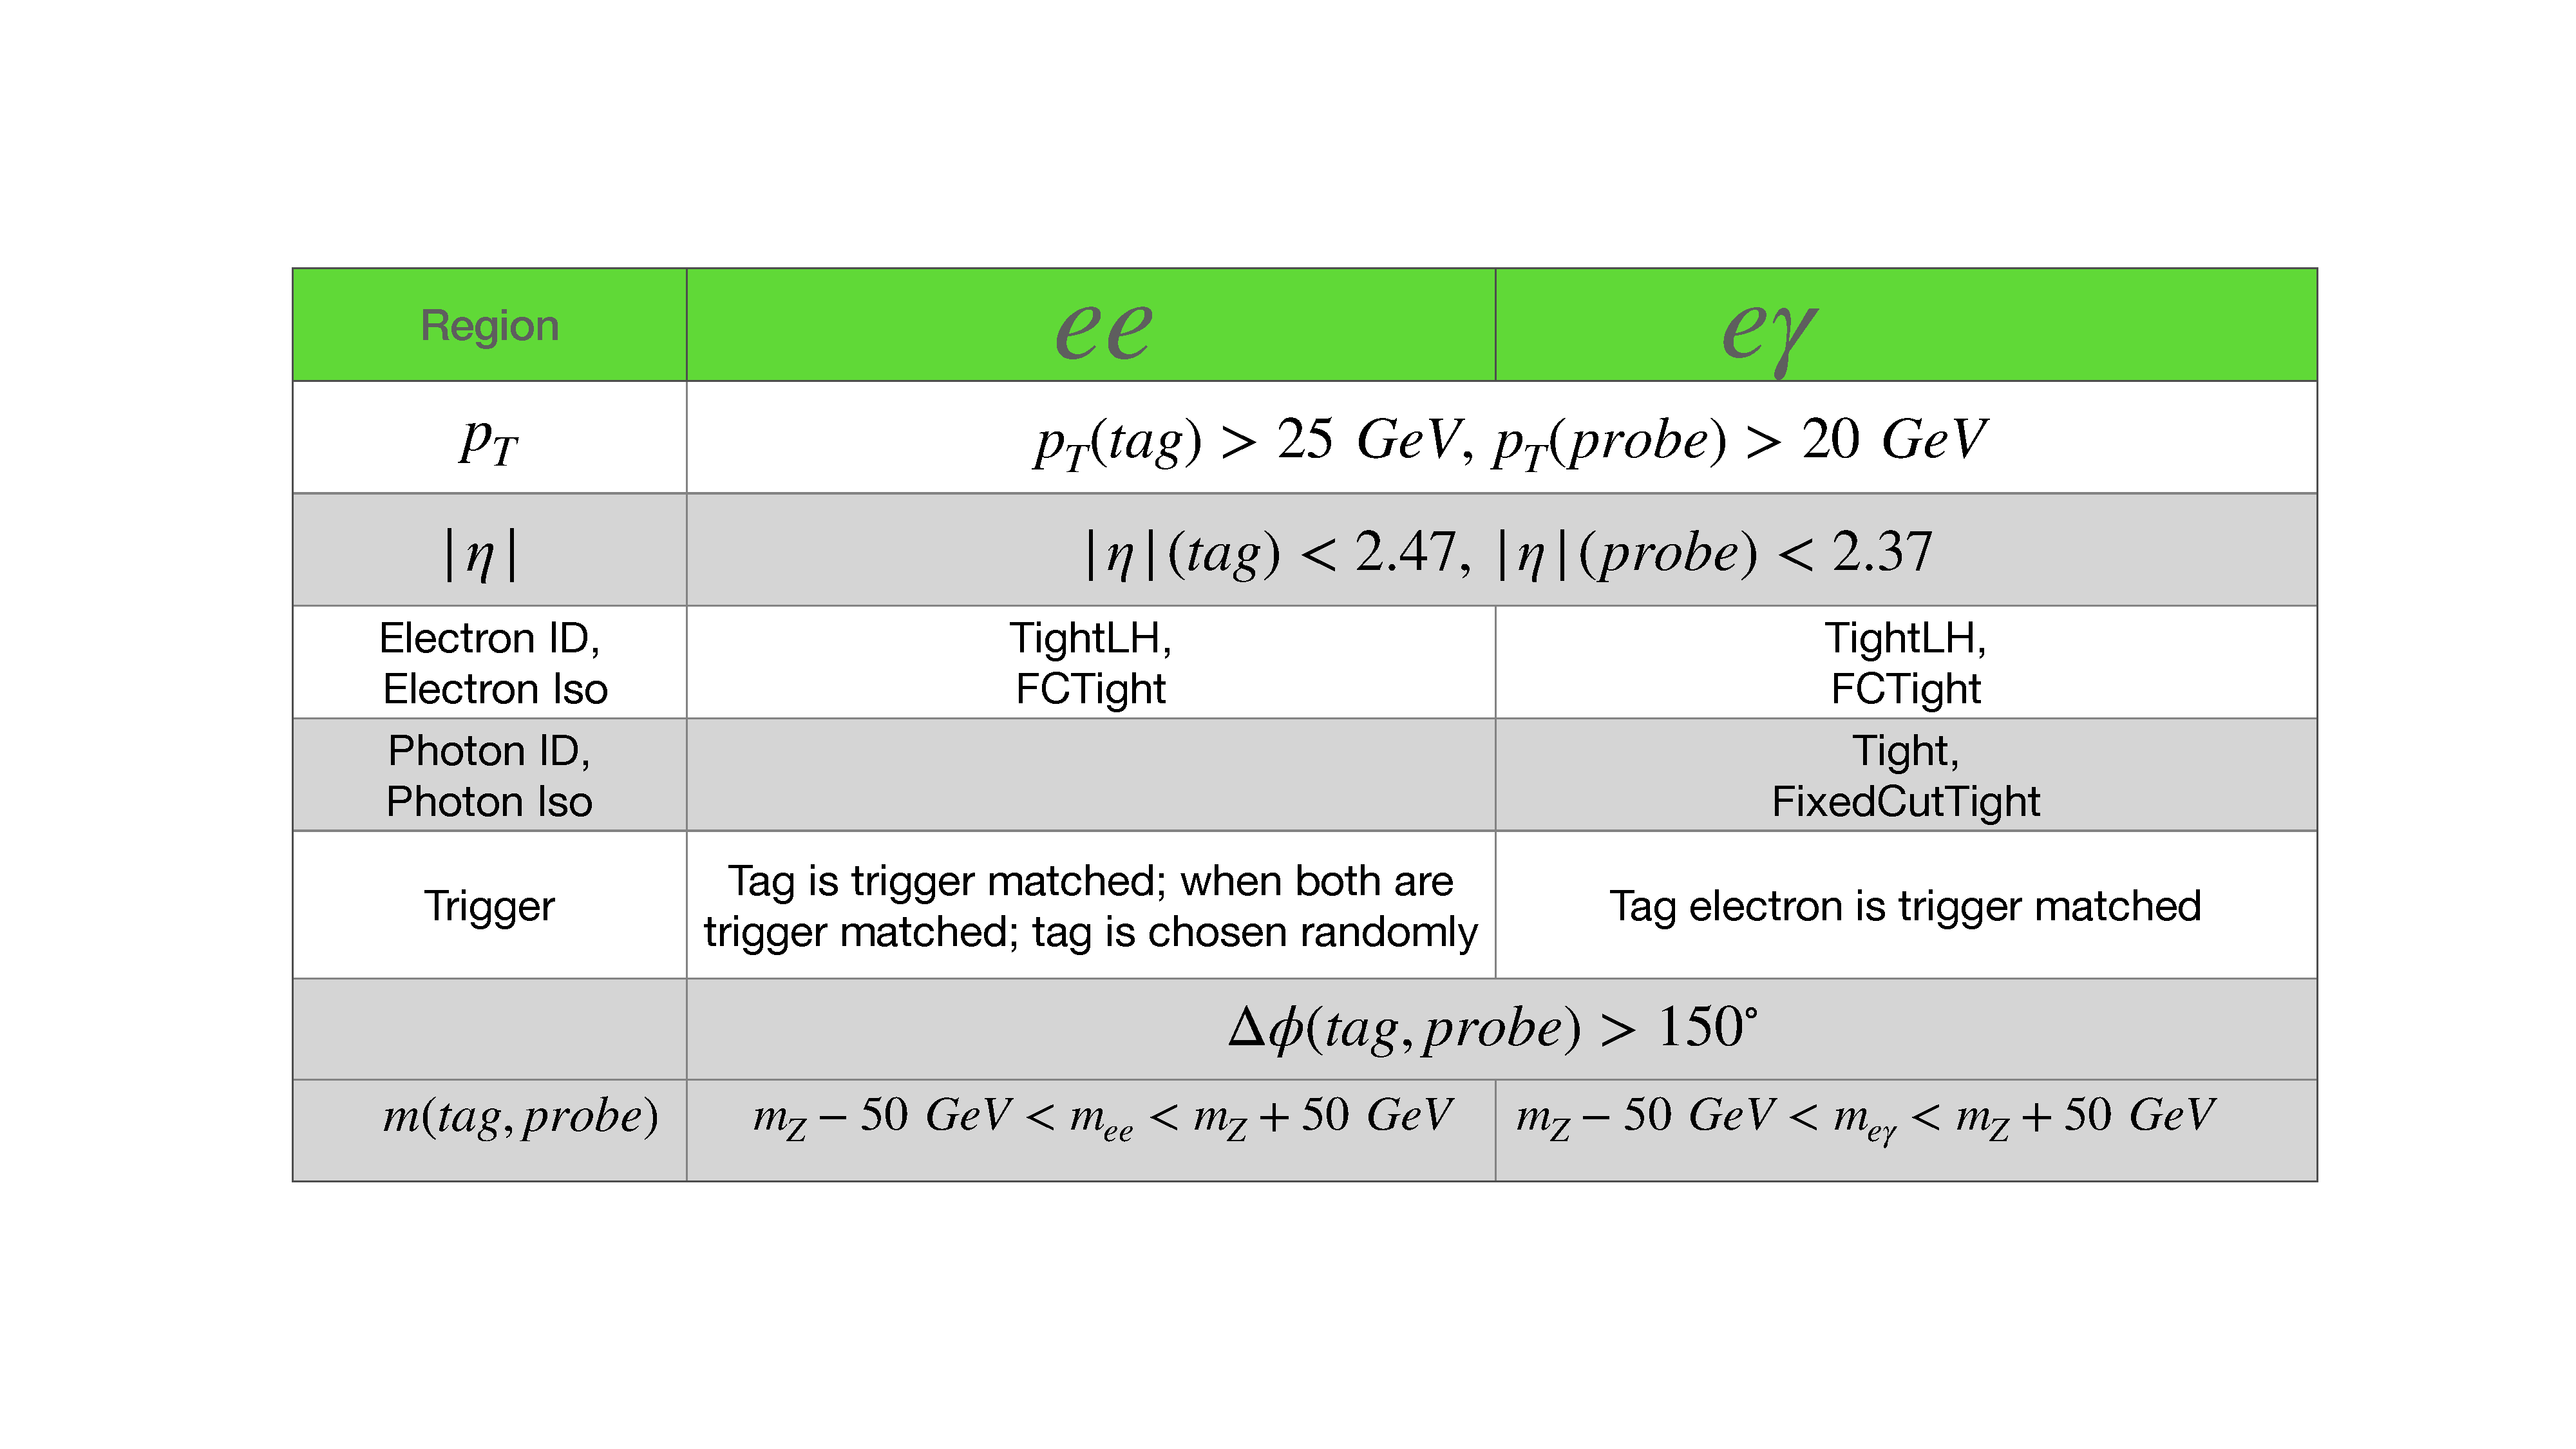
\includegraphics[width=0.69\textwidth]{figures/egammafakes/efakeCR.pdf}}
\caption [] {Definition of $ee$ and $e\gamma$ control regions.}
\label{fig:egammafake_cr}
\end{figure} 

%The cut-flows of these two control region selections are shown in Table~\ref{tab:egammafake_crcutflow} in Appendix~\ref{app:cutflow} for the $Z\to ee$ MC sample, which is expected to be the dominant process in these two control regions.

\FloatBarrier
\subsection{Fake sources}
\label{sec:egammafakes_source}

The $Z\to ee$ MC events selected in the above described $e\gamma$ control region can be used to study the source of $e\to\gamma$ fakes, by matching the probe photon with a truth particle before the detector simulation.
The matching is done by extrapolating the track of the truth particle to the calorimeter layer and calculating the angular distance between the truth particle and the EM cluster, from which the photon is reconstructed.
If the distance is smaller than a reference value ($\Delta R < 0.3$), the truth particle is considered to be the source of the photon.

After truth matching, the photon is categorised into four classes.
\begin{itemize}
\item Type (a): denoted as "mis-reco.", where the photon is matched to a true electron. 87\% of the selected photons belong to this class.
\item Type (b): denoted as "mis-match", where the photon is matched to a true photon, but the photon's \pt is larger than that of the true photon by more than 10\%\footnote{The 10\% threshold is chosen such that it is larger than the photon \pt resolution, of the order of a few percent, and thus such a large difference are expected to arise from a mismatch about the objects.}, and at the same time, there is a nearby true electron with $\Delta R < 0.1$ w.r.t. the photon. 
1.8\% of the selected photons belong to this class.
\item Type (c): denoted as "non-prompt QED", where the photon is matched to a true photon, and their relative \pt difference is smaller than 10\%, although there is a nearby true electron with $\Delta R < 0.1$ w.r.t. the probe photon. 3\% of the selected photons belong to this class. The categorization into type (b) and (c) using the 10\% criterion is only done for illustration purposes to better understand the composition of the fake photons. All three categories (a) -- (c) are considered inclusively as $e\rightarrow \gamma$ fakes. %This categorization is done only for illustration of the impact of different sources.

\item Type (d): denoted as "prompt QED", where the photon is matched to a true photon, and there is no nearby true electron with $\Delta R < 0.1$ w.r.t. the photon. 
8\% of the selected photons belong to this class. 
\end{itemize}
The categorization is summarized in Figure~\ref{fig:egammafake_classes}. The categorization is meant for illustration purposes, all sources of $e\rightarrow \gamma$ fake photons (type(a), type(b) and type(c)) are considered to estimate the fake rate in MC. 


\begin{figure}[!htbp]
\centering
%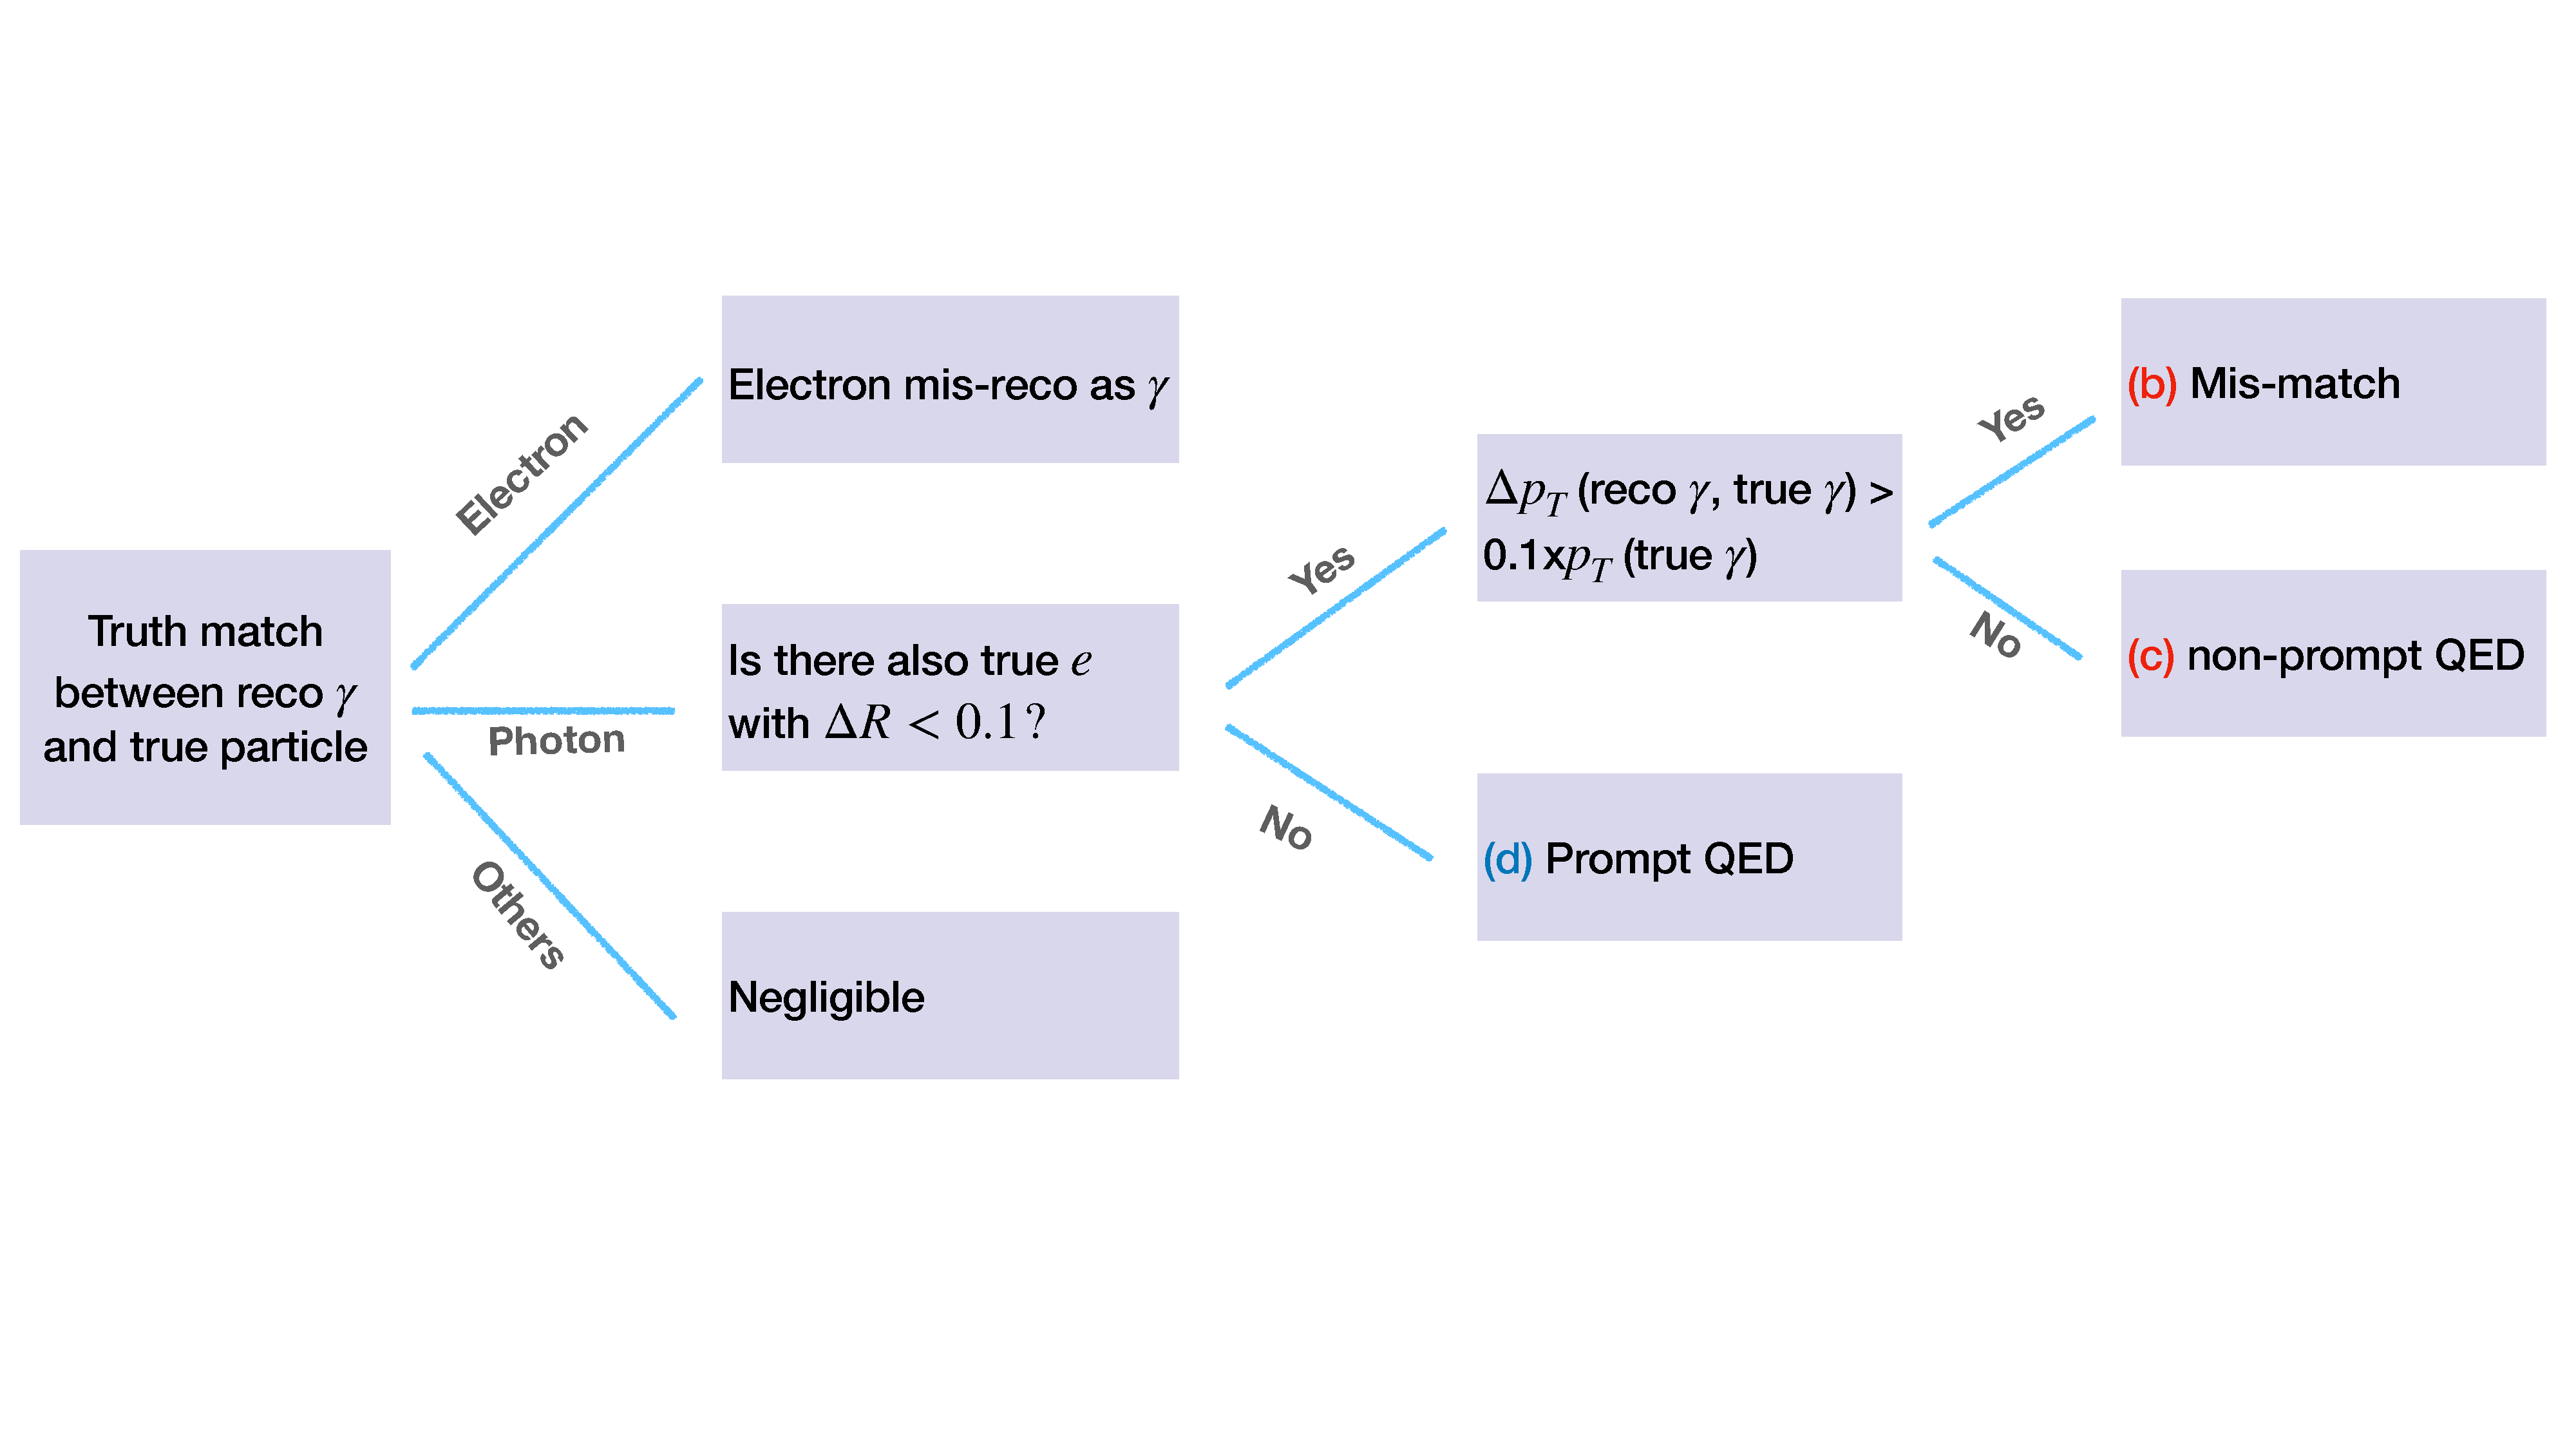
\includegraphics[width=0.49, scale=2.0\textwidth]{figures/egammafakes/efake_truth_matching.pdf}}
{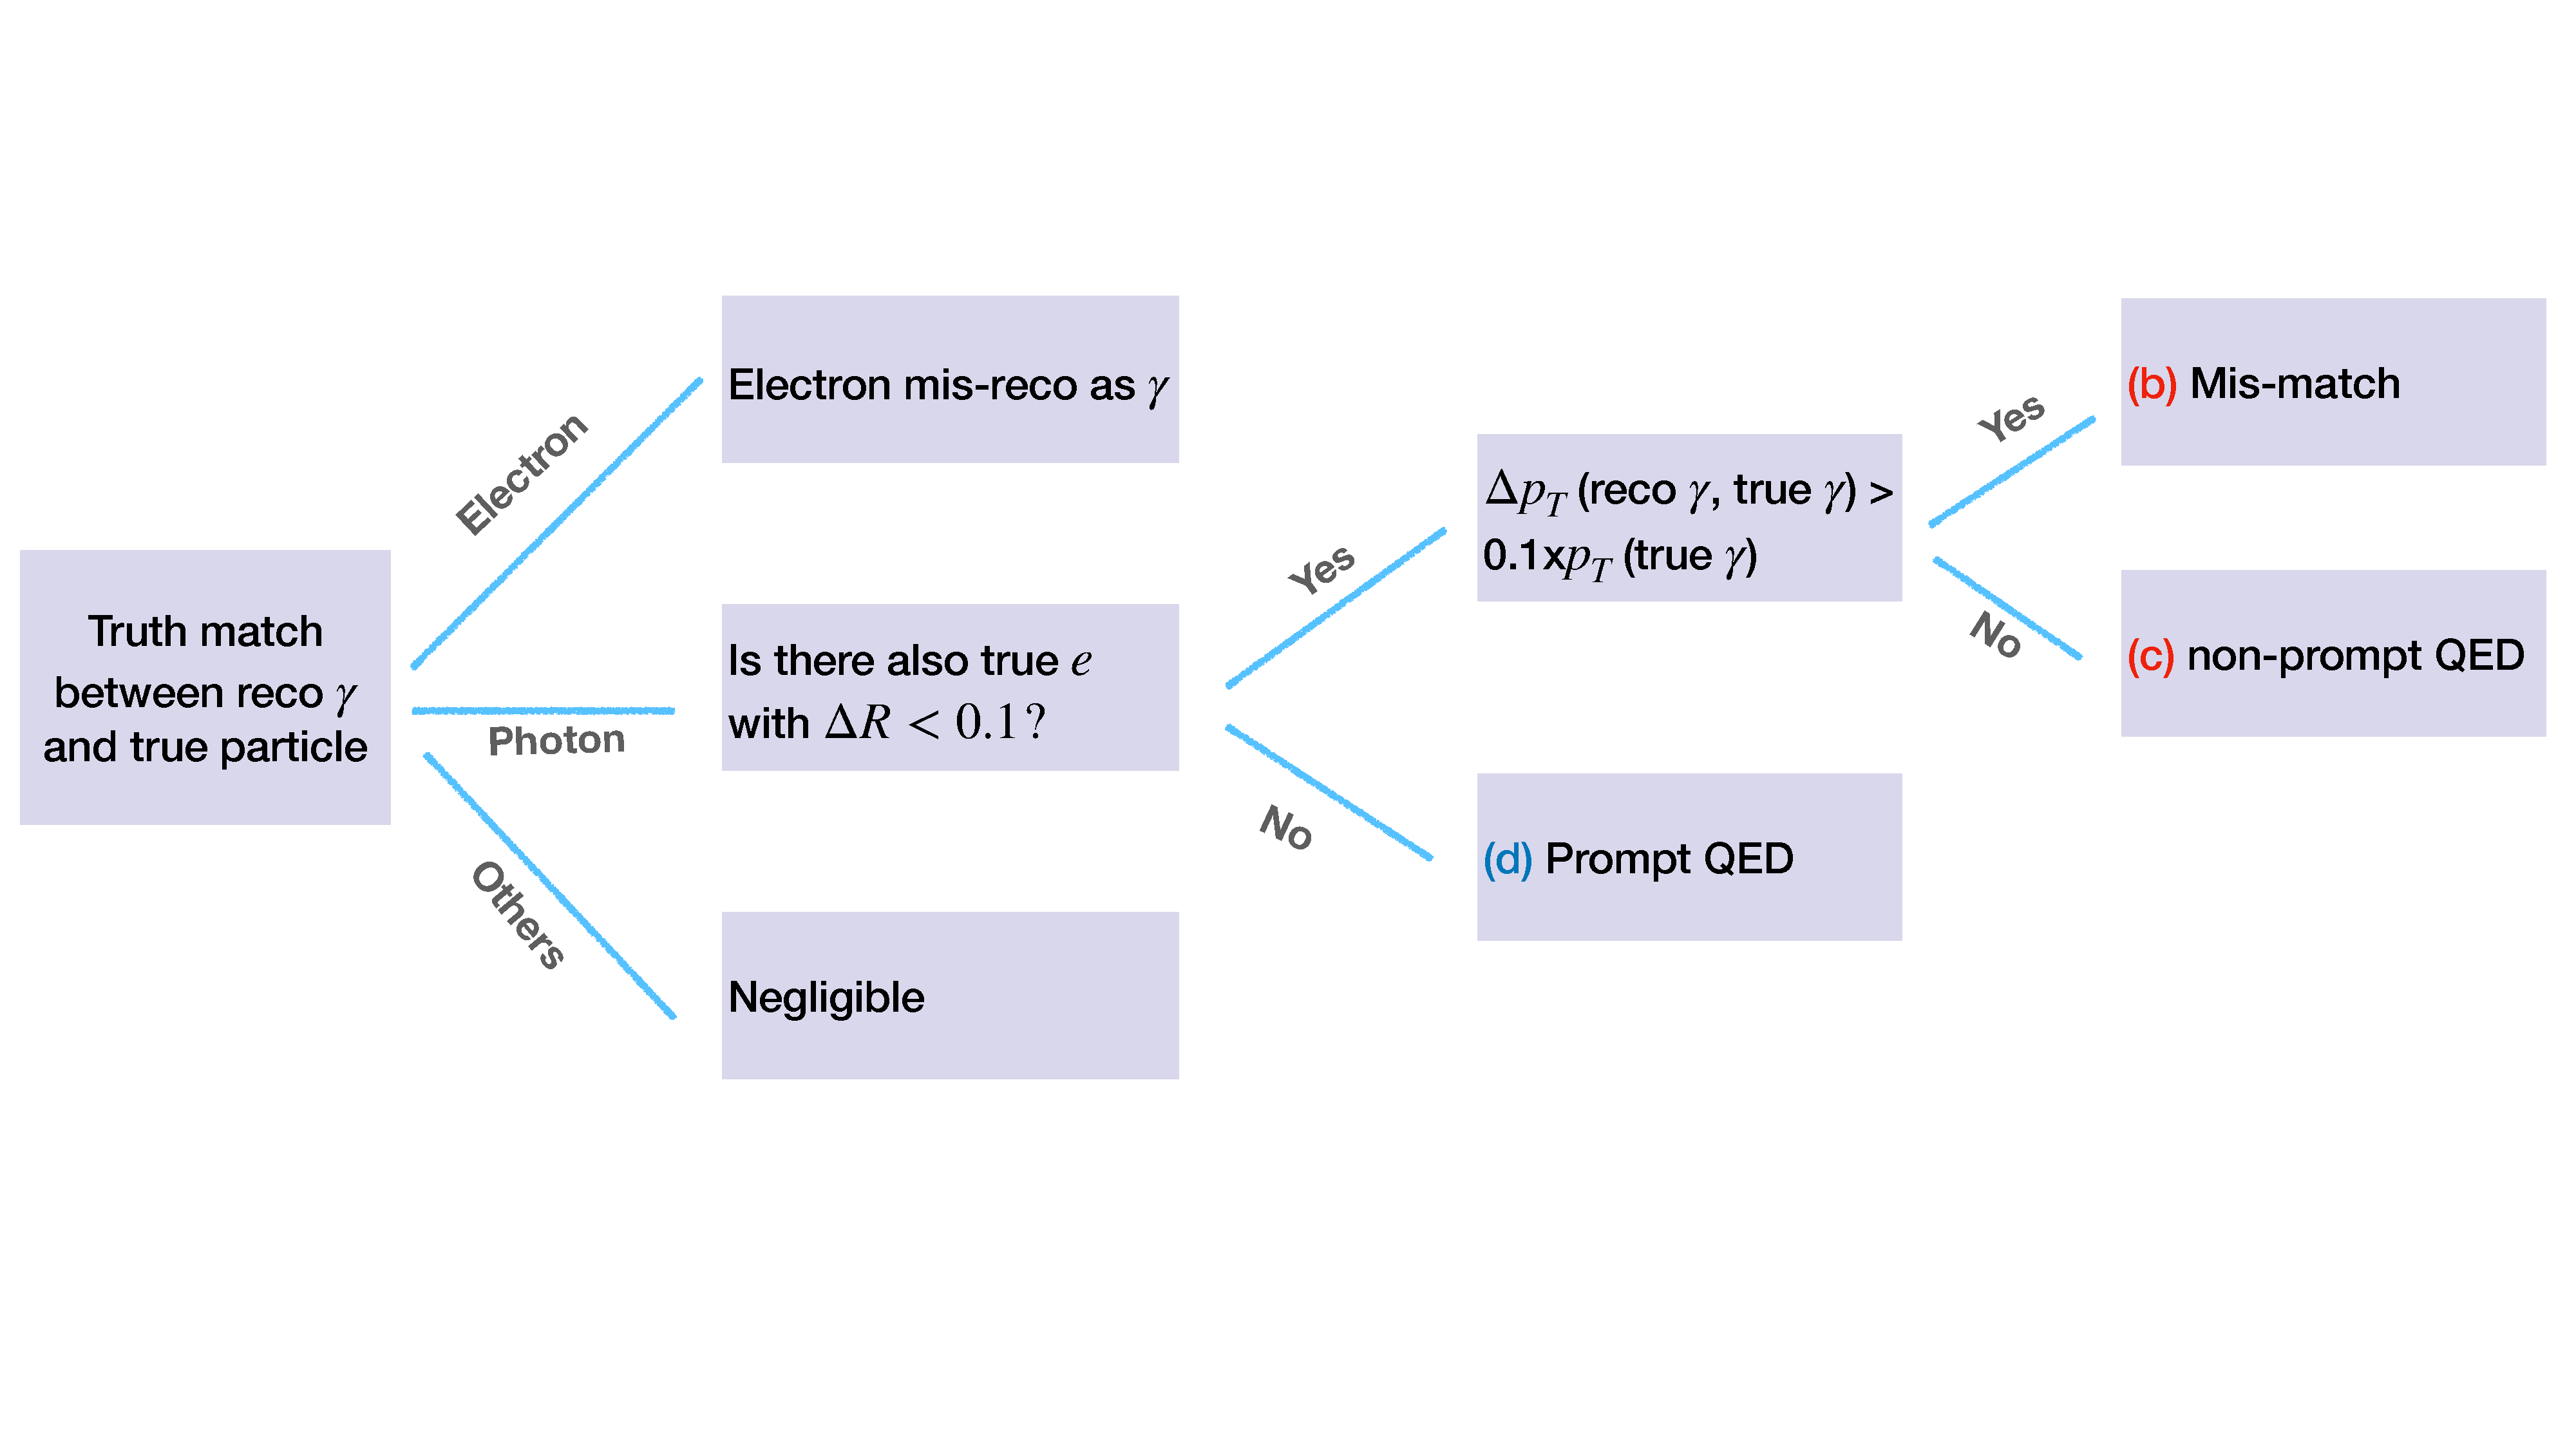
\includegraphics[width=0.69\textwidth]{figures/egammafakes/efake_truth_matching.pdf}}
\caption [] {The categorisation of the selected probe photons in the $e\gamma$ control region via truth particle matching.}
\label{fig:egammafake_classes}
\end{figure}  

In the following, to better understand these four types of photons, their kinematics are shown and compared to that of the probe electron, when available.

The \pt and $\eta$ of the probe photons are compared to those of the probe electron in Figure~\ref{fig:egammafake_probepteta}. 
It can be seen that the \pt spectrum is rather similar between photon type (a), (b), and (c) and the probe electron, which indicates that they are truly $e\to\gamma$ fakes.
For the $\eta$ distribution, type (a) and (b) peak at high $\eta$ region. Connecting to the fact that there is also larger upstream material in high $\eta$ region, it implies (a) and (b) are likely to be bremsstrahlung photons.
For type (c), its $\eta$ spectrum is very similar to that of the probe electron. This could be explained by a very hard non-prompt QED that takes away almost all kinematics of its mother electron.

The invariant mass between the tag and probe in the two control regions are compared in Figure~\ref{fig:egammafake_tagmass}~\subref{fig:efakeInvmassComp}. The lower-shifted mass spectrum for type (d) indicates that it is a true prompt photon from the three body decay of $Z\to e^+e^- +\gamma$. Therefore, type (d) is not to be counted as $e\rightarrow \gamma$ fake. The invariant mass distribution of tag electron and probe photon is shown in Figure~\ref{fig:egammafake_tagmass}~\subref{fig:efakeInvmassStack}, with each type of photons being normalized to their expected yields. It can be seen that the fake is dominated by the type (a).


\begin{figure}[!htbp]
\centering
\subfloat[]{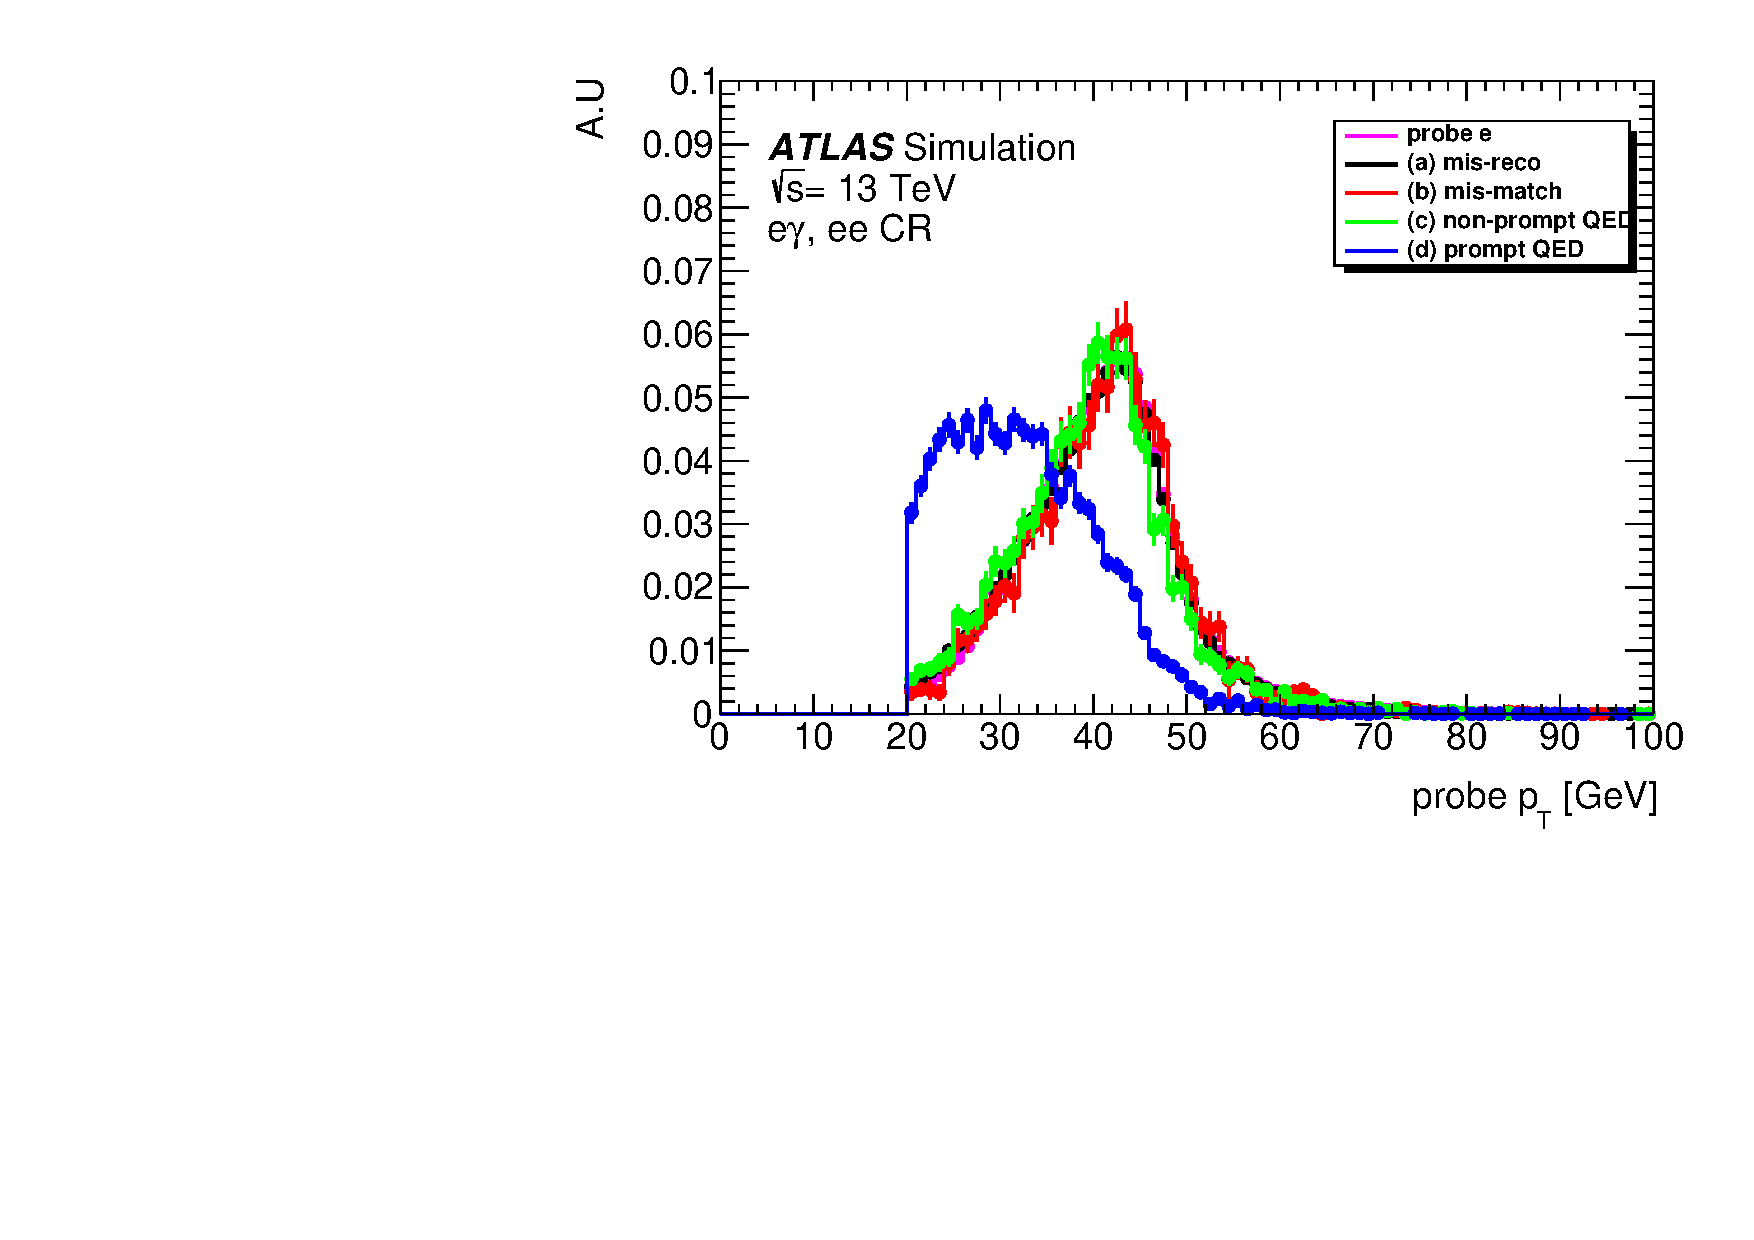
\includegraphics[width=0.49\textwidth]{figures/egammafakes/probe_efake_pt.pdf}}
\subfloat[]{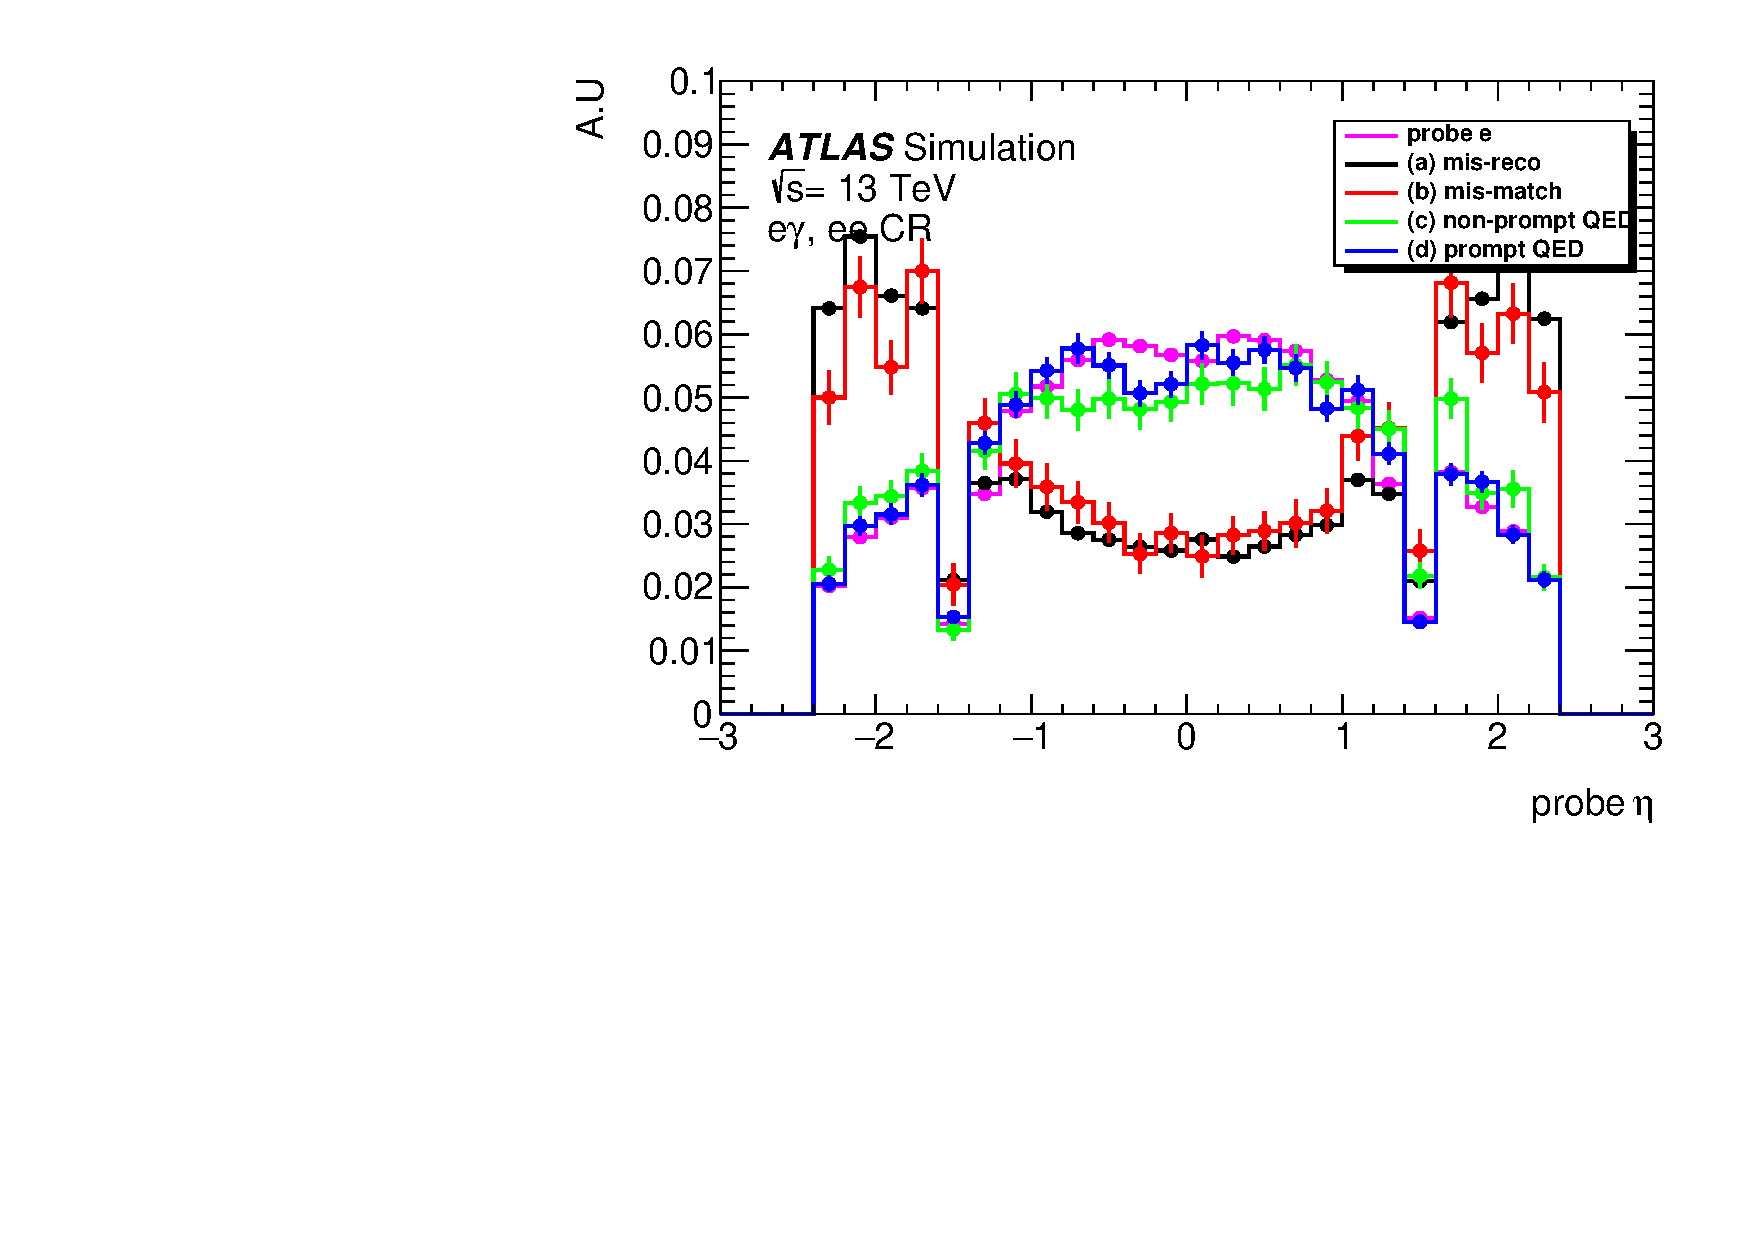
\includegraphics[width=0.49\textwidth]{figures/egammafakes/probe_efake_eta.pdf}}
	\caption [] {The \pt (a) and $\eta$ (b) distributions of different types of probe photon in the $e\gamma$ CRs. The distributions are compared with the kinematic properties of the probe electron in the $ee$ CR. The distributions are obtained using $Z\rightarrow e^+e^-$ MC. In the $e\gamma$ CR most of the photons correspond to a misreconstructed electron. In that case, if the photon in the $e\gamma$ CR corresponds to a misreconstructed electron, then it should have similar kinematic distribution as the probe electron in the $ee$ CR.}
\label{fig:egammafake_probepteta}
\end{figure}   

\begin{figure}[!htbp]
\centering
\subfloat[]{
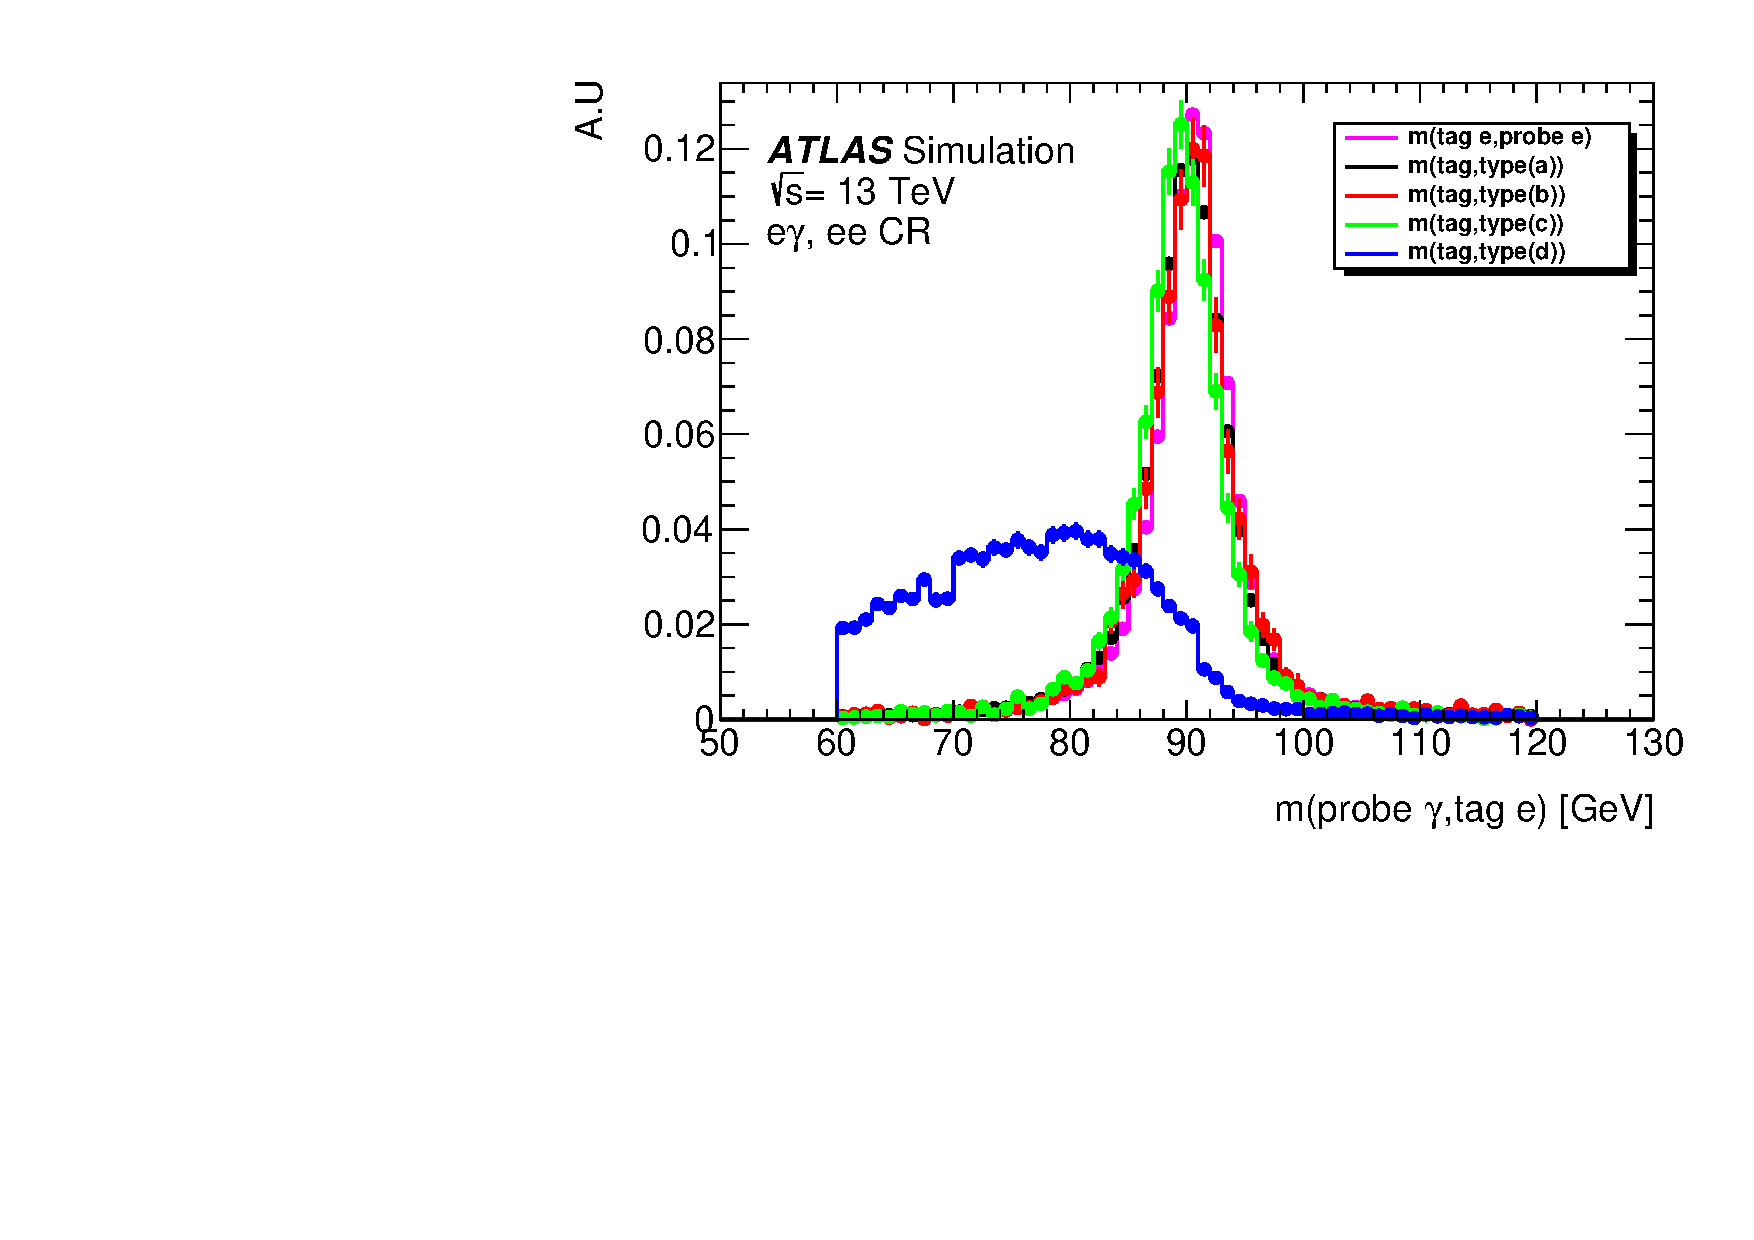
\includegraphics[width=0.49\textwidth]{figures/egammafakes/efake_invmass_comp.pdf}\label{fig:efakeInvmassComp}
}
\subfloat[]{
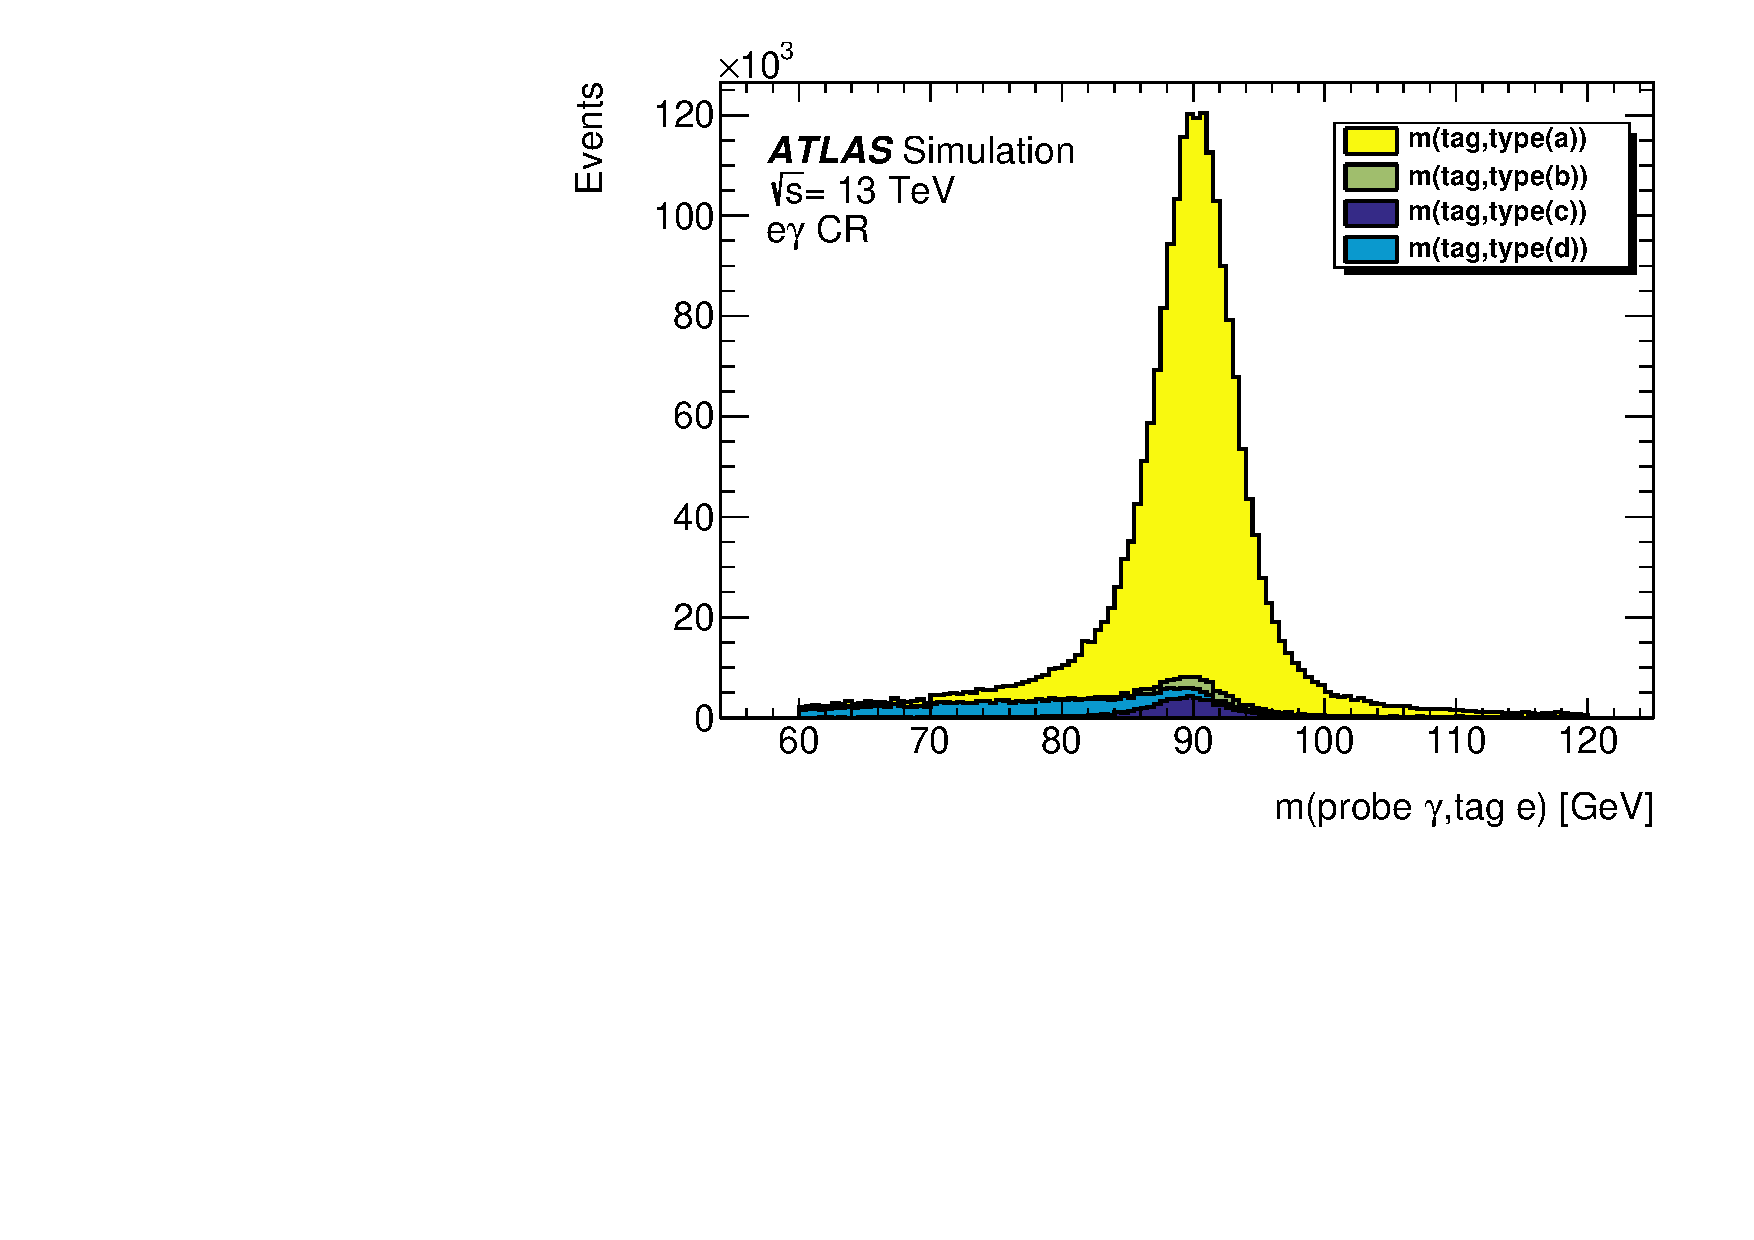
\includegraphics[width=0.49\textwidth]{figures/egammafakes/efake_invmass_stack.pdf}\label{fig:efakeInvmassStack}
}
\caption [] {(a) Normalized invariant mass distribution between the tag and different probe types in the $e\gamma$ and $ee$ CR.(b) The invariant mass between the tag and different probe types in $e\gamma$ CR.}
\label{fig:egammafake_tagmass}
\end{figure} 
  

\FloatBarrier
\subsection{Fake rates}
\label{sec:egammafakes_fr}

Using the $Z\to ee$ MC, the number of $Z\to ee$ events observed with a tag electron in any place and a fake photon in a particular bin can be expressed as follows:
\begin{equation}
N_{e,\gamma}^i = N_{true}^i \times \epsilon_e^{reco} \times \epsilon_e^{\mathrm{others}} \times p_{e\to\gamma}^i \times \epsilon_{\gamma(F)}^i
\end{equation}
where
\begin{itemize}
\item $i$ is the binning index of \pT or $\eta$ or both
\item $N_{true}^i$: true number of generated $Z\to ee$ events where the probe electron is in bin $i$
\item $\epsilon_e^{reco}$ and $\epsilon_e^{\mathrm{others}}$: reconstruction and other selection efficiencies of tag electron
\item $p_{e\to\gamma}^i$: probability of misidentifying an electron as photon in bin $i$
\item $\epsilon_{\gamma}^i(F)$: selection efficiency of the fake photon in bin $i$ ("F" denotes the fact that it's a fake photon so that the efficiency can be different from the true photon)
\end{itemize}

Also, the number of $Z\to ee$ events observed with a tag electron in any place and a probe electron in a particular bin can be expressed as follows:
\begin{equation}
N_{e,e}^i = N_{true}^i \times \epsilon_{e1}^{reco} \times \epsilon_{e1}^{\mathrm{others}} \times \epsilon_{e2}^{reco,i} \times \epsilon_{e2}^{\mathrm{others},i}
\end{equation}
where
\begin{itemize}
\item $\epsilon_{e1}^{reco}$ and $\epsilon_{e1}^{\mathrm{others}}$: reconstruction and other selection efficiencies of tag electron
\item $\epsilon_{e2}^{reco,i}$ and $\epsilon_{e2}^{\mathrm{others},i}$: reconstruction and other selection efficiencies of probe electron in bin $i$
\end{itemize}

The fake rate (FR) in a particular bin $i$ is then defined as the ratio between $N_{e,\gamma}^i$ and $N_{e,e}^i$:
\begin{equation}
\text{FR}^i \equiv \frac{N_{e,\gamma}^i}{N_{e,e}^i} = p_{e\to\gamma}^i \times \frac{\epsilon_{\gamma}^i(F)}{\epsilon_{e2}^{reco,i} \cdot \epsilon_{e2}^{\mathrm{others},i}} = p_{e\to\gamma}^i \times C^i
\end{equation}
From the above formula, it is known that $FR^i$ is proportional to the $e\to\gamma$ faking probability in that bin. The proportion coefficient $C^i$ could also vary.
%nd $\eta$ of the fake candidate, due to the \pt and $\eta$ dependency of those efficiencies.

%An overall fake rate can be calculated using the same formula and its MC value are shown in Table~\ref{tab:egammafake_fr_mc}. 
In Figure~\ref{fig:egammafake_fr_diff}, the \pt and $\eta$ dependencies of the absolute differential fake rate are shown.  
In Figure~\ref{fig:egammafake_fr_diff}, the type (d), which is not really a $e\rightarrow \gamma$ fake photon, is shown for completeness.

%\begin{table}[h]
%\centering
%\caption[]{The overall fake rate calculated from $Z\to ee$ MC for different types of photon. Type (d) is not counted as $e\rightarrow \gamma$ fake photon and its value is just shown for completeness. Only statistical uncertainties are shown here.}
%\vspace*{0.5cm}
%\begin{tabular}{c|c|c|c}
%\hline
%\hline
%& N(probe $\gamma$) & N(probe $e$) & $\text{FR}_{\text{MC}}(\%)$ \\
%\hline
%%	Type(a) & \numRF{1903184.40}{3} $\pm$ \numRF{5493.01}{2} & \numRF{29430386.00}{3} $\pm$ \numRF{20219.12}{2} & \numRF{6.46}{2} \\ \hline 
%%	Type(b) & \numRF{38927.34}{3}   $\pm$ \numRF{754.92}{2}  & \numRF{29430386.00}{3} $\pm$ \numRF{20219.12}{2} & \numRF{0.13}{2} \\ \hline 
%%	Type(c) & \numRF{65791.93}{3}   $\pm$ \numRF{946.80}{2}  & \numRF{29430386.00}{3} $\pm$ \numRF{20219.12}{2} & \numRF{0.22}{2}\\ \hline 
%%	Type(d) & \numRF{170667.31}{3}  $\pm$ \numRF{1549.72}{2} & \numRF{29430386.00}{3} $\pm$ \numRF{20219.12}{2} & \numRF{0.58}{2} \\ \hline 
%%	All     & \numRF{2178570.98}{3} $\pm$ \numRF{5834.48}{2} & \numRF{29430386.00}{3} $\pm$ \numRF{20219.12}{2} & \numRF{7.40}{2}\\ \hline 
%\hline
%\end{tabular}
%\label{tab:egammafake_fr_mc}
%\end{table}

\begin{figure}[!htbp]
\centering
\subfloat[]{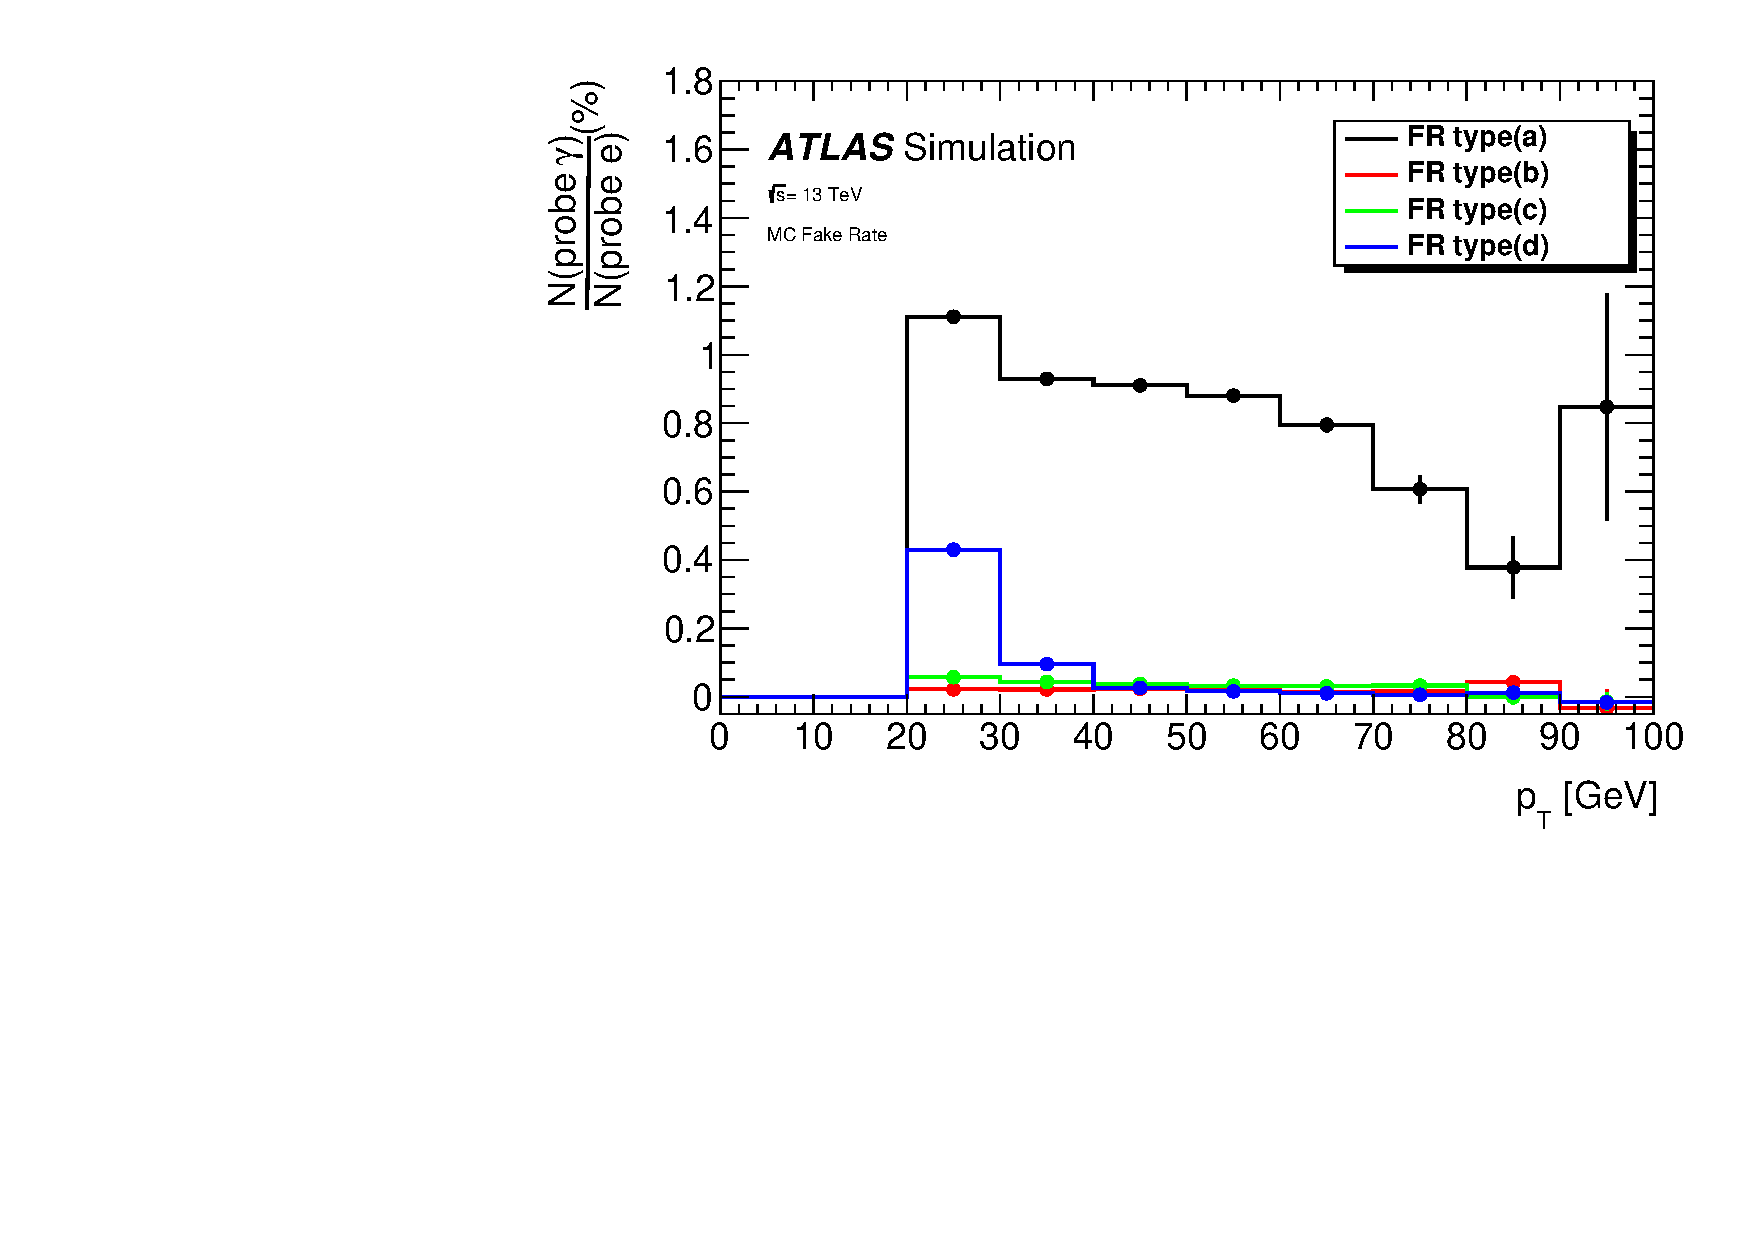
\includegraphics[width=0.49\textwidth]{figures/egammafakes/efake_rate_pt.pdf}}
\subfloat[]{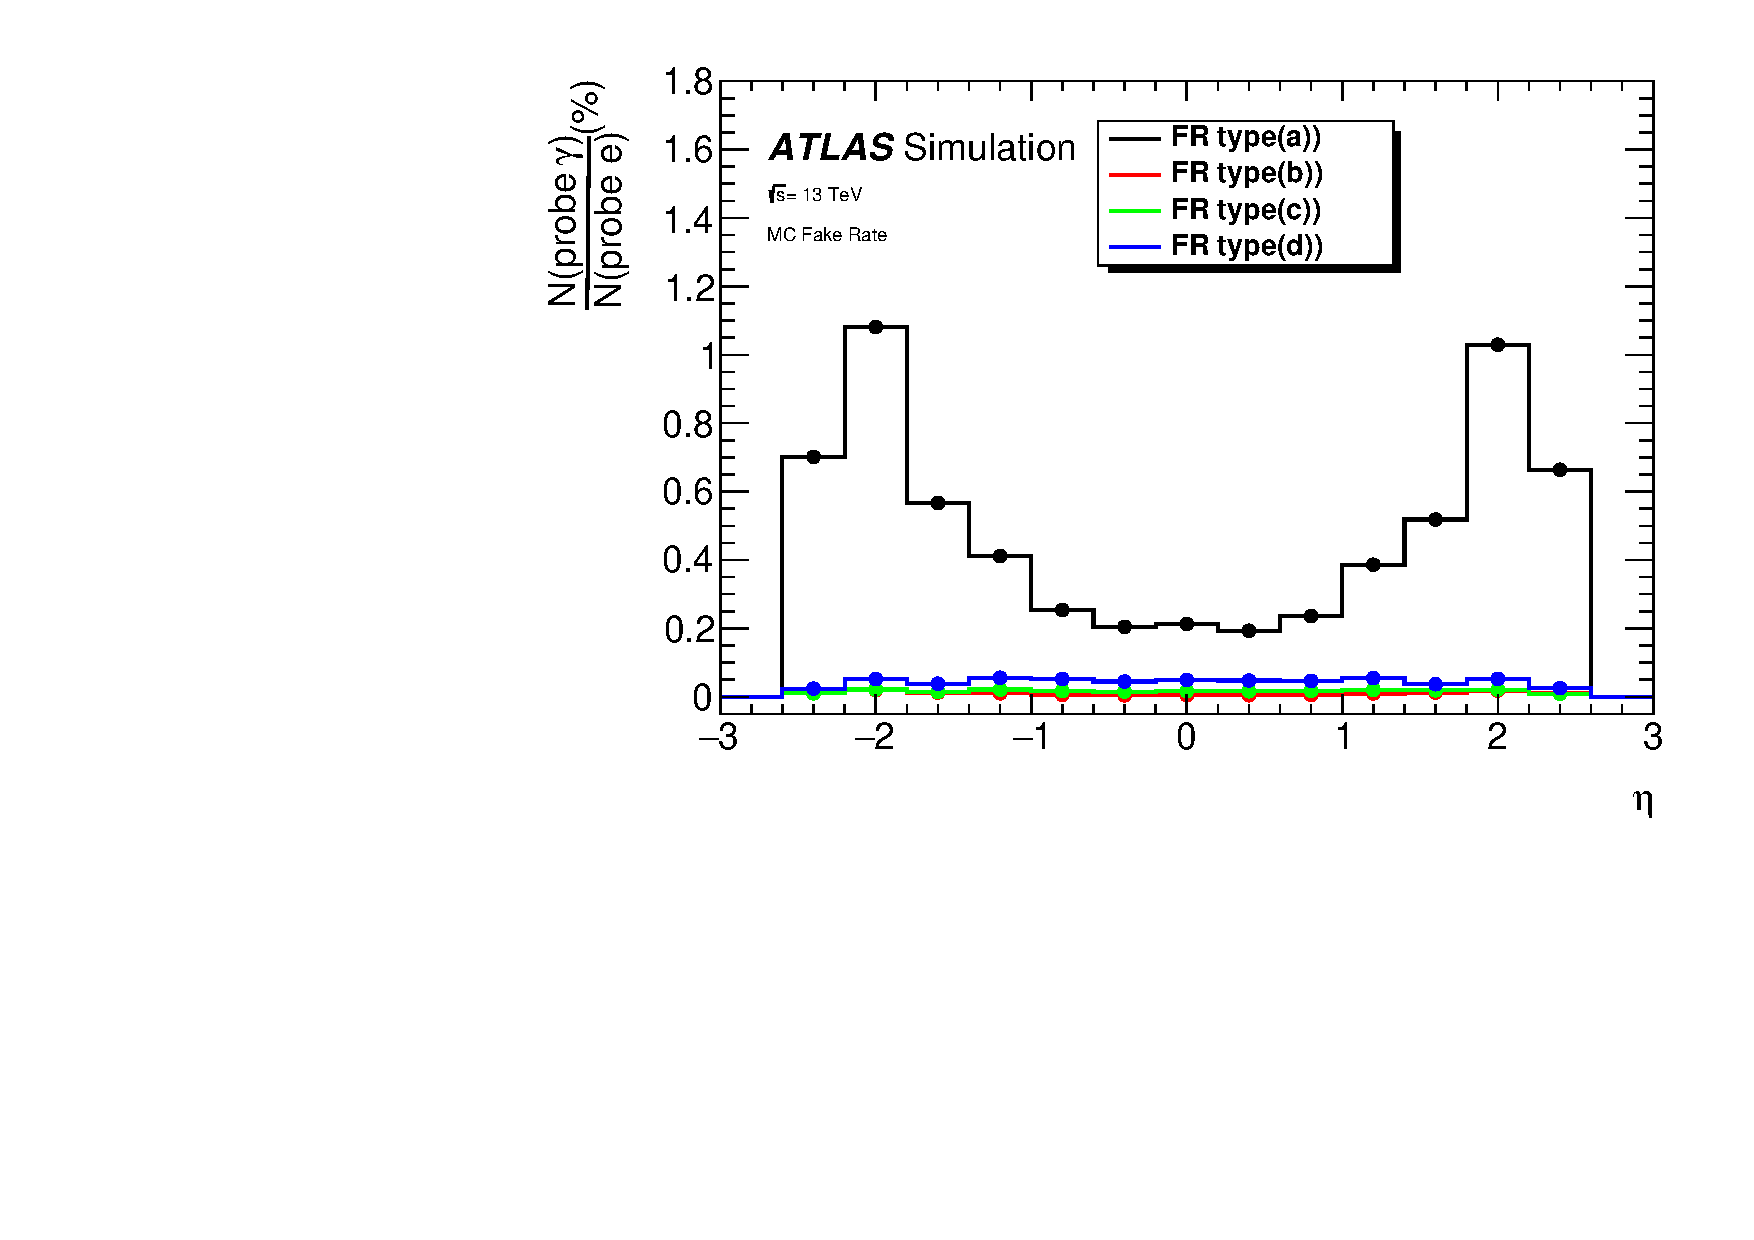
\includegraphics[width=0.49\textwidth]{figures/egammafakes/efake_rate_eta.pdf}}
\caption [] {The \pt (a) and $\eta$ (b) dependency of the fake rates}
\label{fig:egammafake_fr_diff}
\end{figure}   

In order to calculate the data-driven fake rate in bin $i$, the only difference with respect to the above MC-based fake rate is that:
\begin{equation}
\text{FR}_{dd}^i = \frac{N_{e,\gamma}^{\mathrm{data},i} - N_{e,\gamma}^{non\text{-}Z,i} - \mathrm{prompt\ QED}}{N_{e,e}^{\mathrm{data},i} - N_{e,e}^{non\text{-}Z,i} - \mathrm{prompt\ QED}}
\end{equation}
which means the denominator and numerator are replaced by their data-driven ones. 

The subtraction of non-$Z$ events from data in these control regions can't be done with MC samples since from MC study the non-$Z$ background are negligible.
Instead, it is done by side band fit,
where the $Z\to ee$ signal is modelled by double-sided Crystal-ball function and the non-$Z$ background by a Bernstein 4th order polynomial. The prompt contribution is subtracted from the data based on the MC template (type(d) photons) before the fit is performed.

After that the data-driven fake rate in bin $i$ is divided by the corresponding MC fake rate to derive a set of fake rate scale factors:
\begin{equation}
\text{SF}_{\text{FR}}^i = \frac{\text{FR}_{dd}^i}{\text{FR}_{MC}^i}
\end{equation}
these scale factors will be applied to the $e\to\gamma$ MC samples as a data-driven correction.

The scale factor is derived in photon $p_T$ and $\eta$ separately for converted and unconverted photons. It is shown in Figure~\ref{fig:egammafake_ptetadiff_sfs_conv} and Figure~\ref{fig:egammafake_ptetadiff_sfs_unconv}. The choice of binning for \pt is [25, 35, 45, 1000] (in GeV) and for $\eta$ is [0, 0.6, 1.37] and [1.52, 1.8, 2.37]. So in the end, there will be $3\times4 = 12$ bins.
%The nominal mass peak fits for each of these bins are shown in Figure \ref{fig:egammafake_fit_ptetadiff_eg} and Figure \ref{fig:egammafake_fit_ptetadiff_ee}.


\vspace*{0.5cm}

To estimate the systematic uncertainty of the scale factor, the following variations are considered: 
\begin{itemize}
\item signal function shape is changed from double sided Crystal-ball to MC predicted template (if necessary with smoothing to reduce fluctuation), the result of which is shown in Figure~\ref{fig:egammafake_fit_syst_converted}~\subref{fig:egammafake_fit_temp_converted} for the converted photon case and in Figure~\ref{fig:egammafake_fit_syst_unconverted}~\subref{fig:egammafake_fit_temp_unconverted} for the unconverted photon case. %We see a difference of 3.7\% (for converted photon) and 4.6\% (for unconverted photon) in the SF value with respect to the nominal SF value.  
%The scale factor is calculated to be 1.14, with a difference of 17\% with respect to the nominal SF.
\item fitting mass range shrunk by 5 GeV in the low end and 5 GeV in the high end, the result of which is shown in Figure~\ref{fig:egammafake_fit_syst_converted}~\subref{fig:egammafake_fit_range_dn_converted} for the converted photon case and in Figure~\ref{fig:egammafake_fit_syst_unconverted}~\subref{fig:egammafake_fit_range_dn_unconverted} for the unconverted photon case. %We see a difference of 2.5\% (for converted photon) and 5.5\% (for unconverted photon) in the SF value with respect to the nominal SF value. 
%The scale factor is calculated to be 1.08, with a difference of 11\% with respect to the nominal SF.
\item background function shape is changed from Bernstein to Gaussian, the result of which is shown in Figure~\ref{fig:egammafake_fit_syst_converted}~\subref{fig:egammafake_fit_bkg_converted} for the converted photon case and in Figure~\ref{fig:egammafake_fit_syst_unconverted}~\subref{fig:egammafake_fit_bkg_unconverted} for the unconverted photon case. %We see a difference of 1.7\% (for converted photon) and 4.6\% (for unconverted photon) in the SF value with respect to the nominal SF value. 
%The scale factor is calculated to be 1.04, with a difference of 7\% with respect to the nominal SF.
%\item the MC model for the subtraction of prompt QED contribution is changed from $Z\to ee$ sample to a $Z\to ee\gamma$ sample.
%The scale factor is calculated to be 0.99, with a difference of 2\% with respect to the nominal SF.
\end{itemize}

The impact of different systematic variations in each $[p_{T};|\eta|]$ bin is shown in Figure~\ref{fig:impact_of_uncertainty_converted} for converted photon case and in Figure~\ref{fig:impact_of_uncertainty_unconverted} for unconverted photon case.

%----------------------------------- sample syst plots for converted photons ------------------------------------------
\begin{figure}[!htbp]
\centering
\subfloat[]{
\includegraphics[width=0.40\textwidth]{figures/egammafakes/converted_ph/syst_sig_var/Zee_fit_eta1pt1.pdf}
\includegraphics[width=0.40\textwidth]{figures/egammafakes/converted_ph/syst_sig_var/Zeg_fit_eta1pt1.pdf}\label{fig:egammafake_fit_temp_converted}
}
\quad
\subfloat[]{
\includegraphics[width=0.40\textwidth]{figures/egammafakes/converted_ph/syst_mass_var/Postfit_Zpeak_PtBin1_EtaBin1_zee.pdf}
\includegraphics[width=0.40\textwidth]{figures/egammafakes/converted_ph/syst_mass_var/Postfit_Zpeak_PtBin1_EtaBin1_zeg.pdf}\label{fig:egammafake_fit_range_dn_converted}
}
\quad
\subfloat[]{
\includegraphics[width=0.40\textwidth]{figures/egammafakes/converted_ph/syst_bkg_var/Postfit_Zpeak_PtBin1_EtaBin1_zee.pdf}
\includegraphics[width=0.40\textwidth]{figures/egammafakes/converted_ph/syst_bkg_var/Postfit_Zpeak_PtBin1_EtaBin1_zeg.pdf}\label{fig:egammafake_fit_bkg_converted}
}
\caption [] {The side band fit in the two control regions to subtract non-$Z$ events, where the signal function is switched from double-sided crystal ball to MC template (a), the fit range is shortened by 10~GeV(b), or the background function is switched from 4th order Bernstein polynomial to Gaussian (c). The above fits are only for a particular pt and eta bin. The above plots are for converted photon case.}
\label{fig:egammafake_fit_syst_converted}
\end{figure} 
%----------------------------------- end sample syst plots for converted photons ------------------------------------------

%----------------------------------- sample syst plots for unconverted photons ------------------------------------------
\begin{figure}[!htbp]
\centering
\subfloat[]{
\includegraphics[width=0.40\textwidth]{figures/egammafakes/unconverted_ph/syst_sig_var/Zee_fit_eta1pt1.pdf}
\includegraphics[width=0.40\textwidth]{figures/egammafakes/unconverted_ph/syst_sig_var/Zeg_fit_eta1pt1.pdf}\label{fig:egammafake_fit_temp_unconverted}
}
\quad
\subfloat[]{
\includegraphics[width=0.40\textwidth]{figures/egammafakes/unconverted_ph/syst_mass_var/Postfit_Zpeak_PtBin1_EtaBin1_zee.pdf}
\includegraphics[width=0.40\textwidth]{figures/egammafakes/unconverted_ph/syst_mass_var/Postfit_Zpeak_PtBin1_EtaBin1_zeg.pdf}\label{fig:egammafake_fit_range_dn_unconverted}
}
\quad
\subfloat[]{
\includegraphics[width=0.40\textwidth]{figures/egammafakes/unconverted_ph/syst_bkg_var/Postfit_Zpeak_PtBin1_EtaBin1_zee.pdf}
\includegraphics[width=0.40\textwidth]{figures/egammafakes/unconverted_ph/syst_bkg_var/Postfit_Zpeak_PtBin1_EtaBin1_zeg.pdf}\label{fig:egammafake_fit_bkg_unconverted}
}
\caption [] {The side band fit in the two control regions to subtract non-$Z$ events, where the signal function is switched from double-sided crystal ball to MC template (a), the fit range is shortened by 5~GeV(b), or the background function is switched from 4th order Bernstein polynomial to Gaussian (c). The above fits are only for a particular pt and eta bin. The above plots are for unconverted photon case.}
\label{fig:egammafake_fit_syst_unconverted}
\end{figure} 

The final 2D scale factors are summarized in Figure~\ref{fig:egammafake_ptetadiff_sfs_conv} and Figure~\ref{fig:egammafake_ptetadiff_sfs_unconv}, including statistical uncertainties as well as the above systematic uncertainties. The SFs obtained in different regions of jet multiplicity were found to be compatible well within the statistical uncertainties, therefore, they are used in both the lepton+jets and dilepton channels.

%---------------------------------------------- efake SF for converted photon ---------------------------
\begin{figure}[!htbp]
\centering
{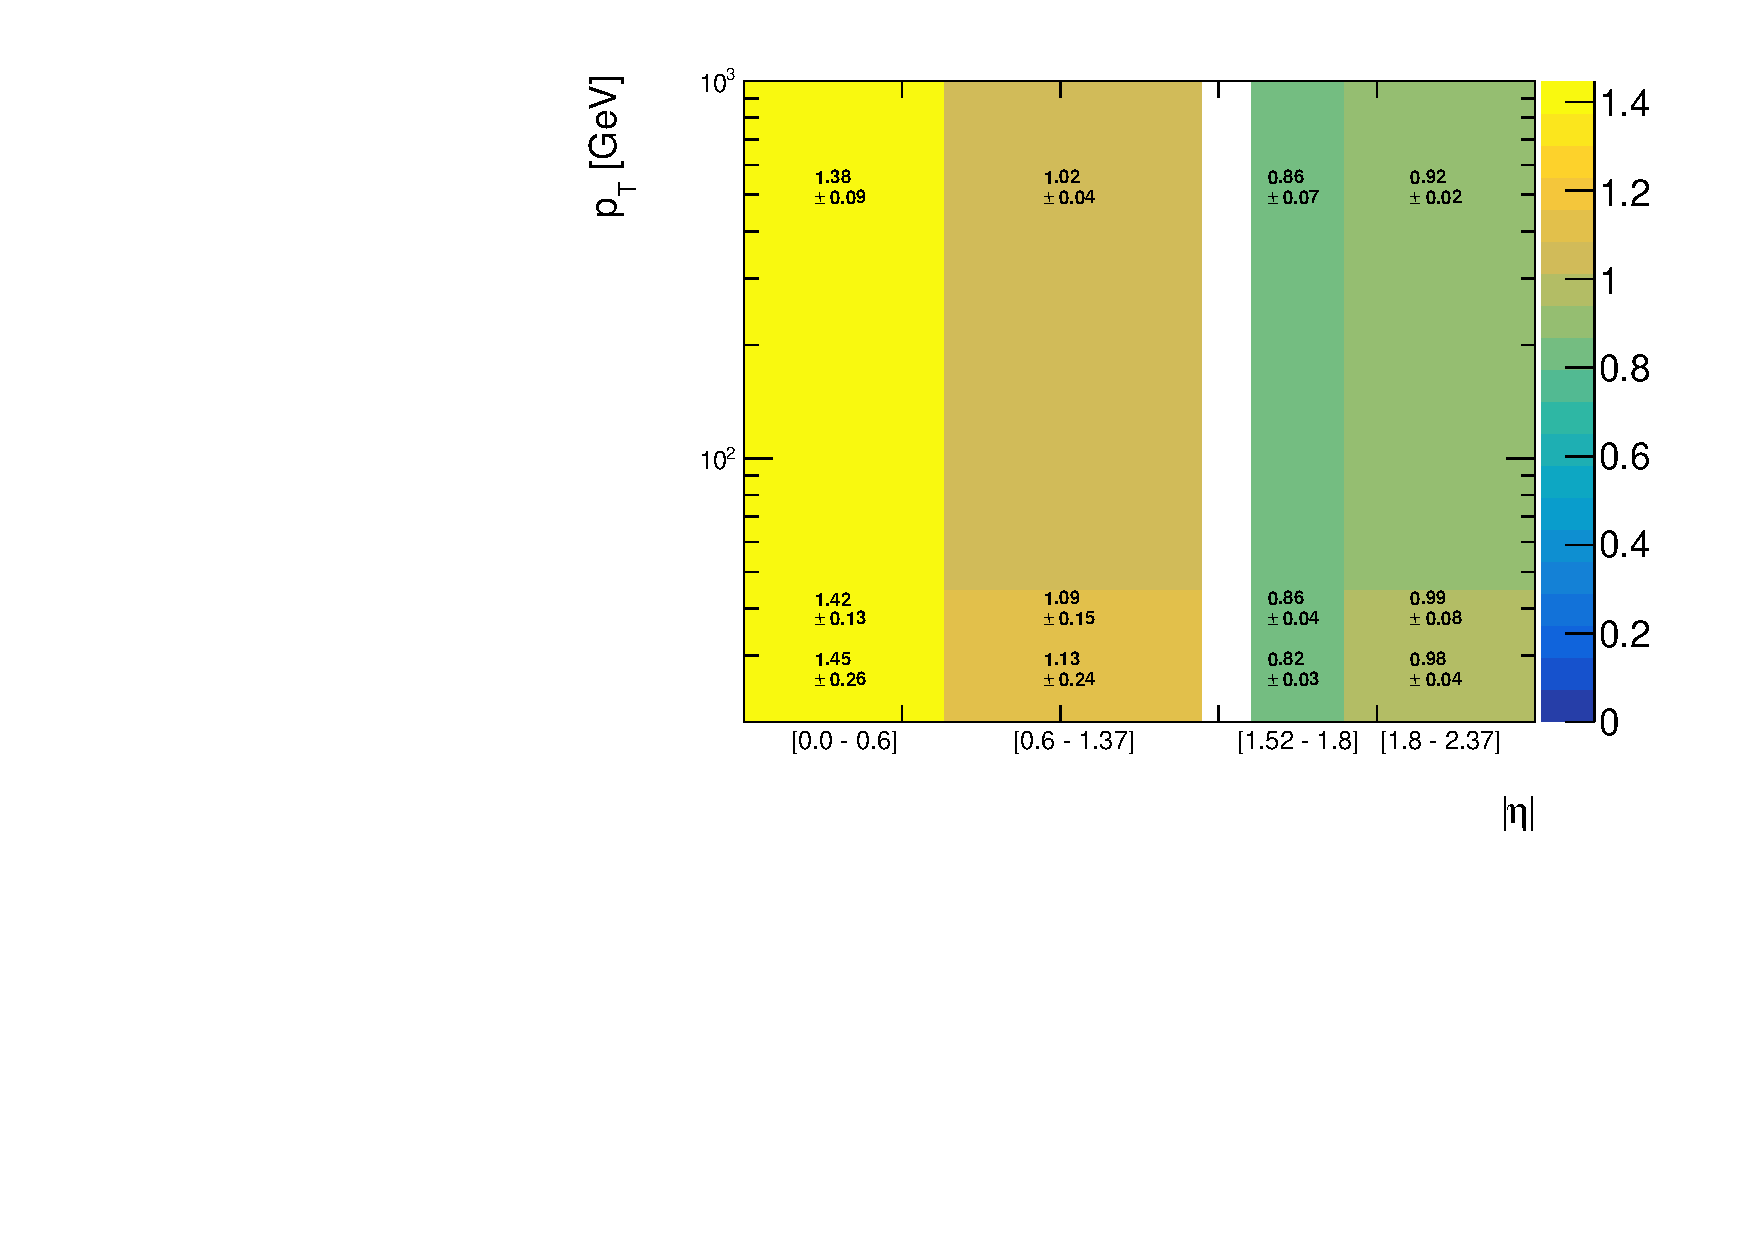
\includegraphics[width=0.7\textwidth]{figures/egammafakes/Map_EFake_SF_Final_converted.pdf}}
\caption [] {The final 2D fake rate scale factors with all uncertainties included (for converted photons).}
\label{fig:egammafake_ptetadiff_sfs_conv}
\end{figure}   
%---------------------------------------------- end efake SF for converted photon ---------------------------

%---------------------------------------------- efake SF for unconverted photon ---------------------------
\begin{figure}[!htbp]
\centering
{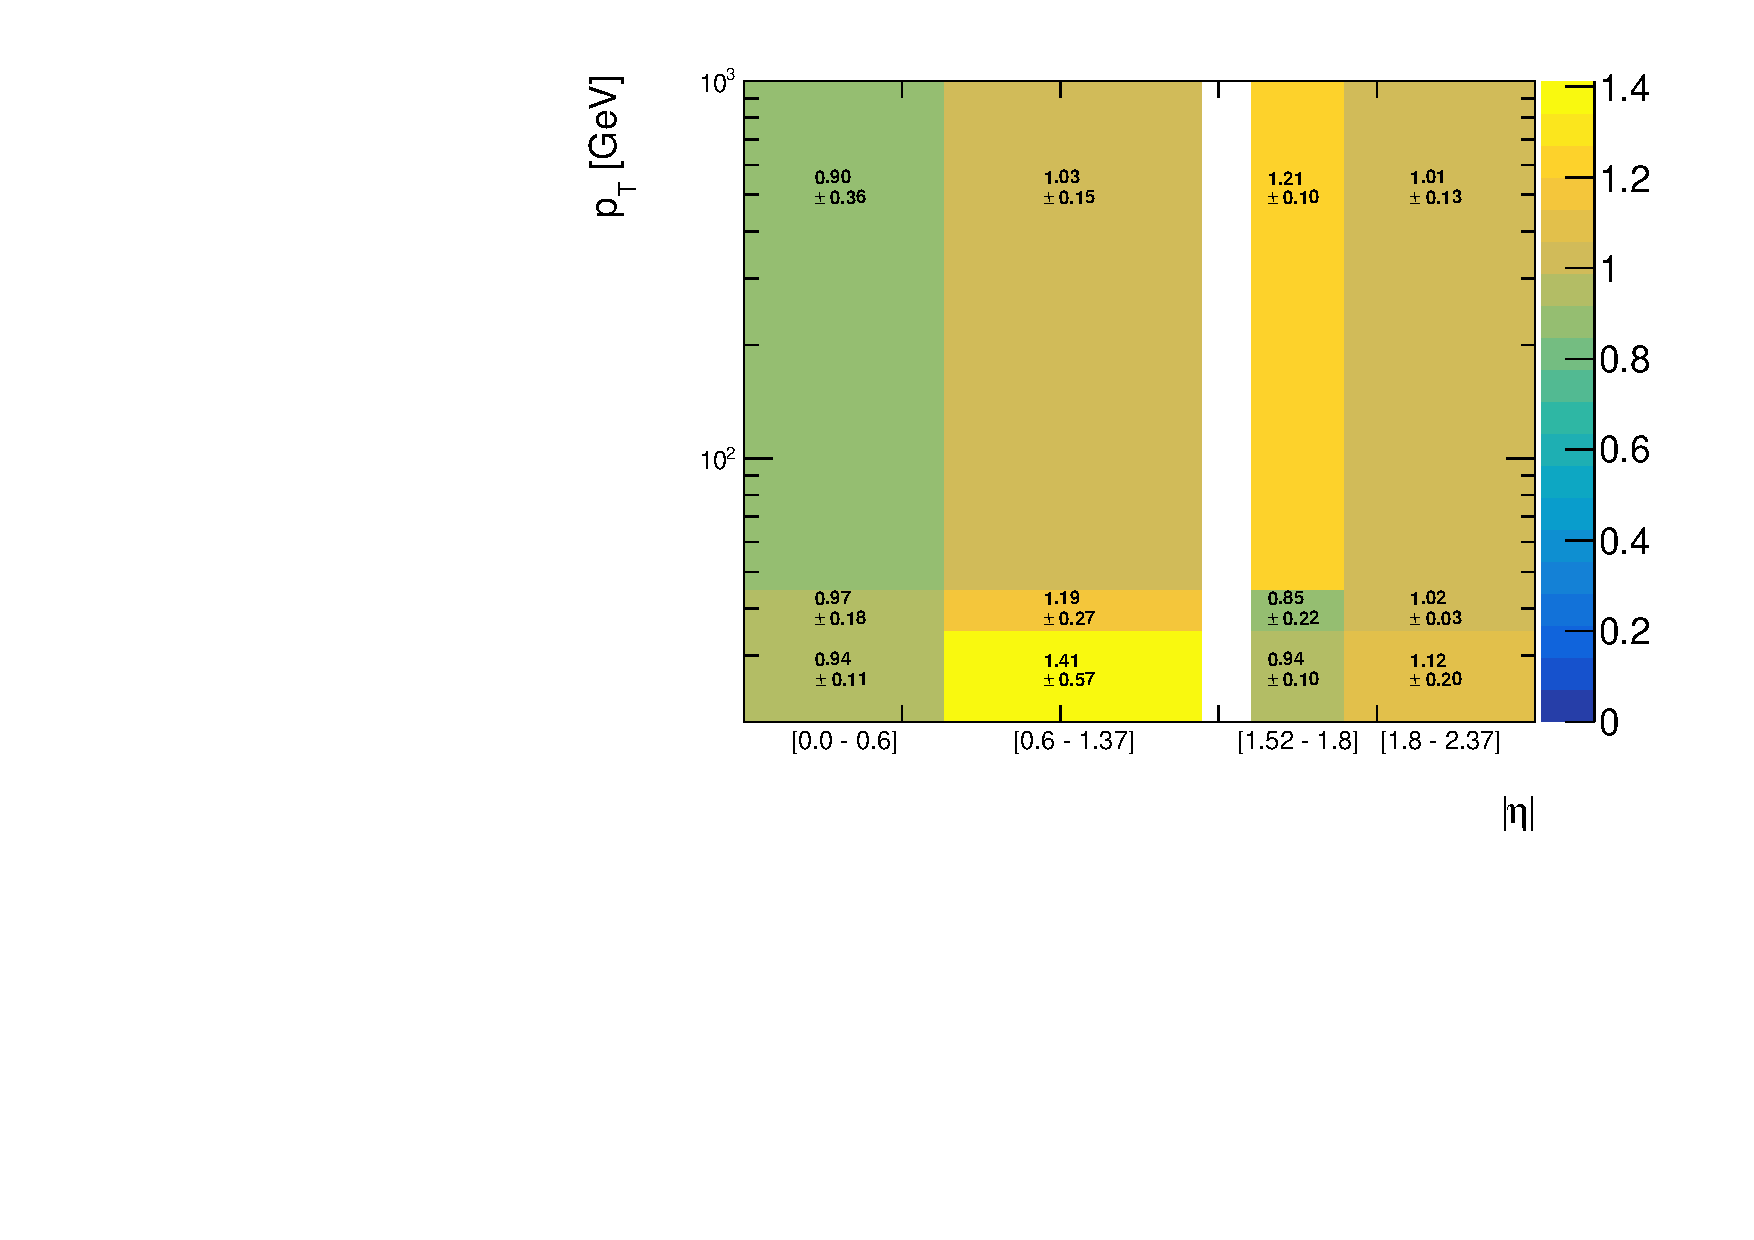
\includegraphics[width=0.7\textwidth]{figures/egammafakes/Map_EFake_SF_Final_unconverted.pdf}}
\caption [] {The final 2D fake rate scale factors with all uncertainties included (for unconverted photon).}
\label{fig:egammafake_ptetadiff_sfs_unconv}
\end{figure}   
%---------------------------------------------- end efake SF for unconverted photon ---------------------------

%--------------------------------------- impact of syst in SF -------------------------
\begin{figure}[!htbp]
\centering
\subfloat[]{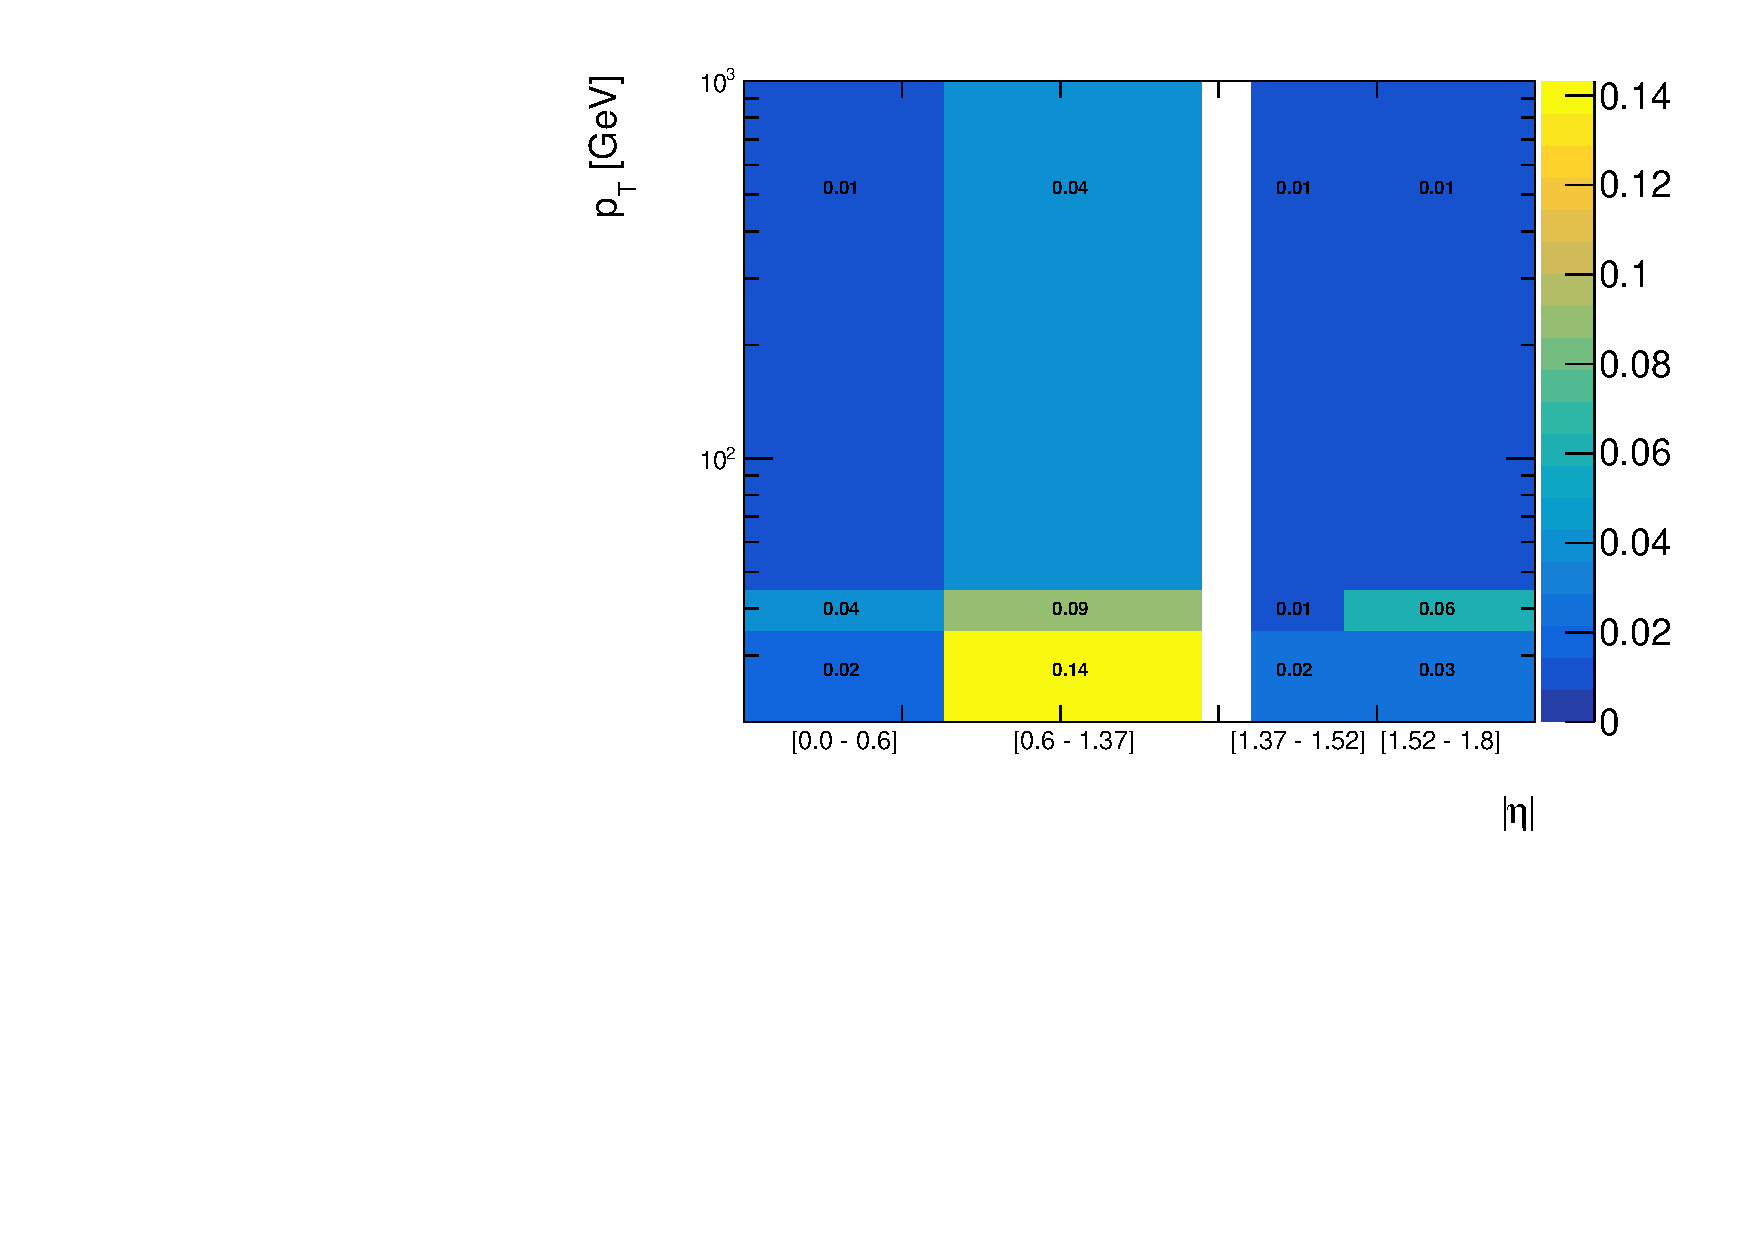
\includegraphics[width=0.45\textwidth]{figures/egammafakes/diffchangingSigtoMCtemplate.pdf}}
\subfloat[]{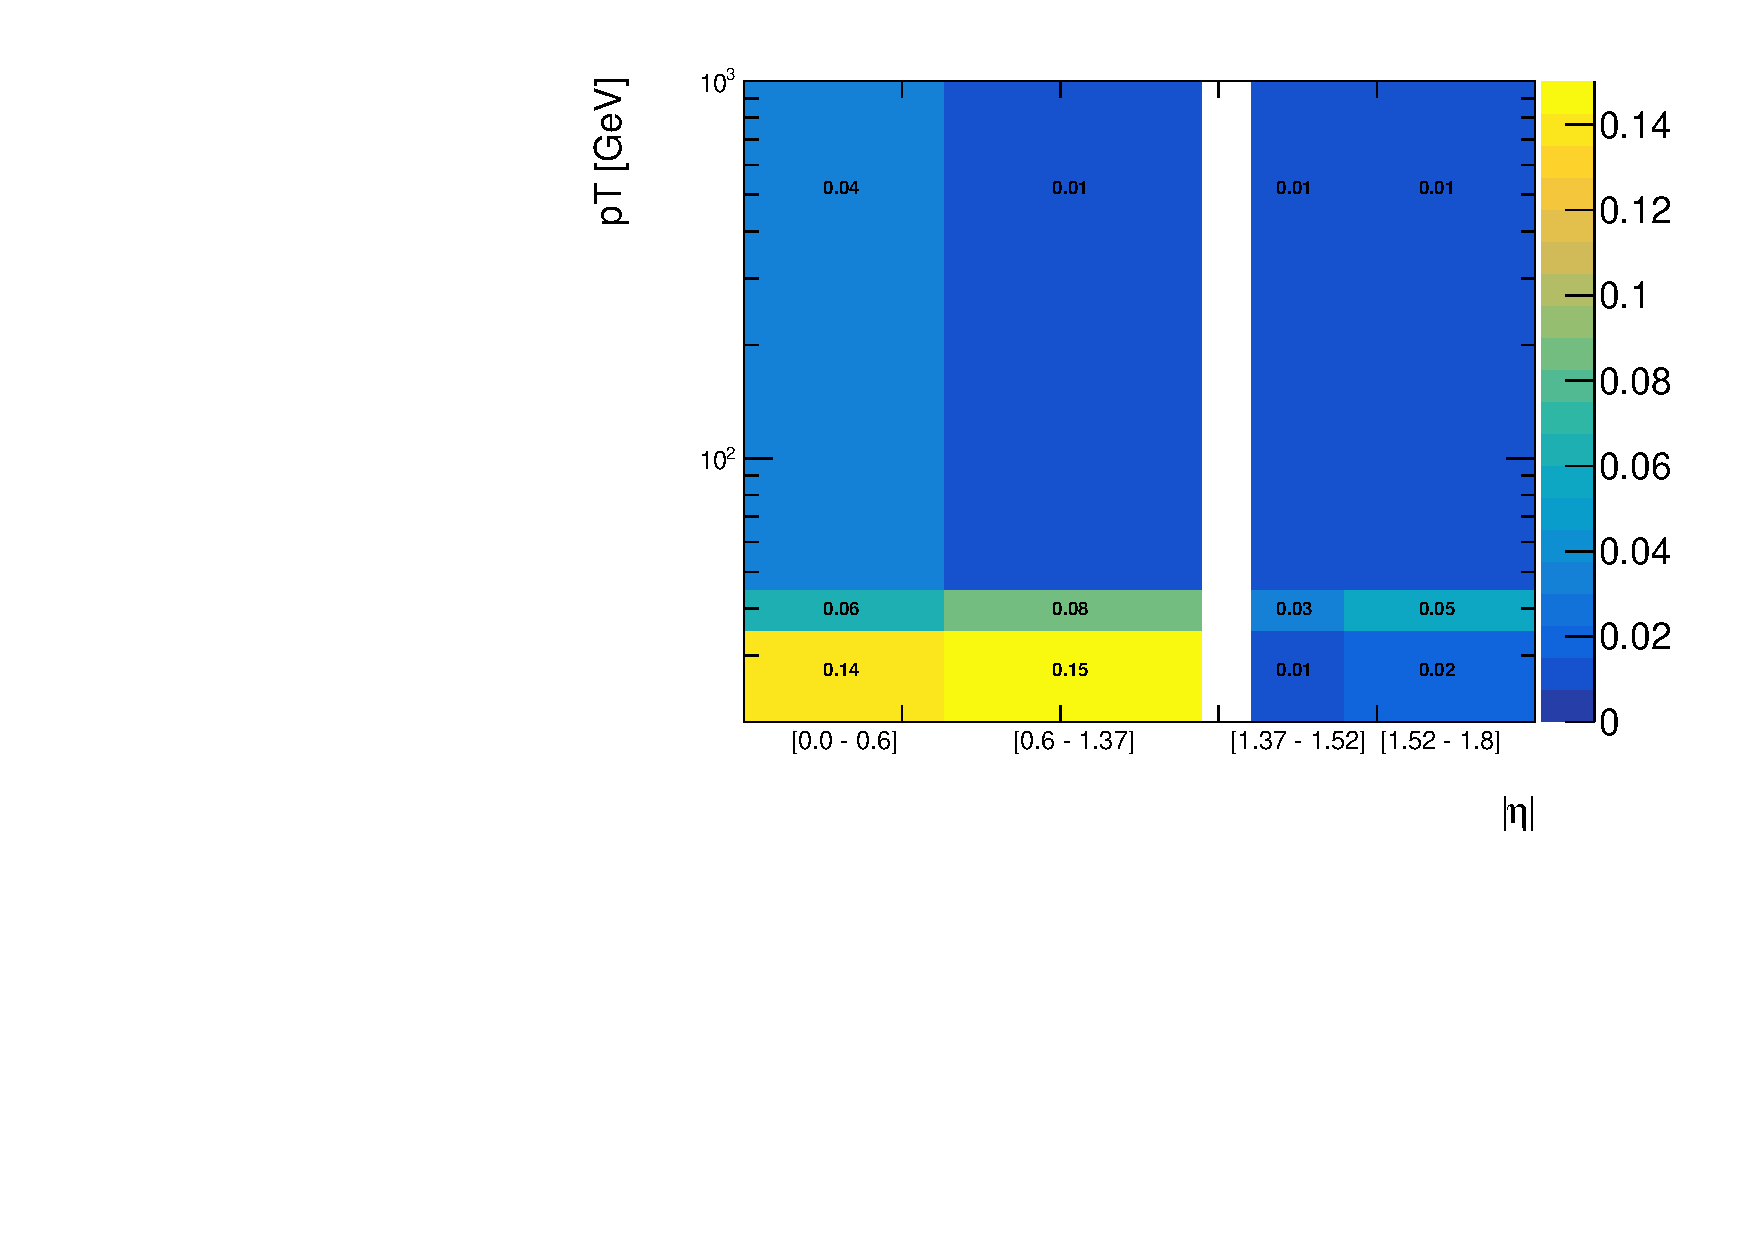
\includegraphics[width=0.45\textwidth]{figures/egammafakes/diffchangingBkgtoGaus.pdf}}
\quad
\subfloat[]{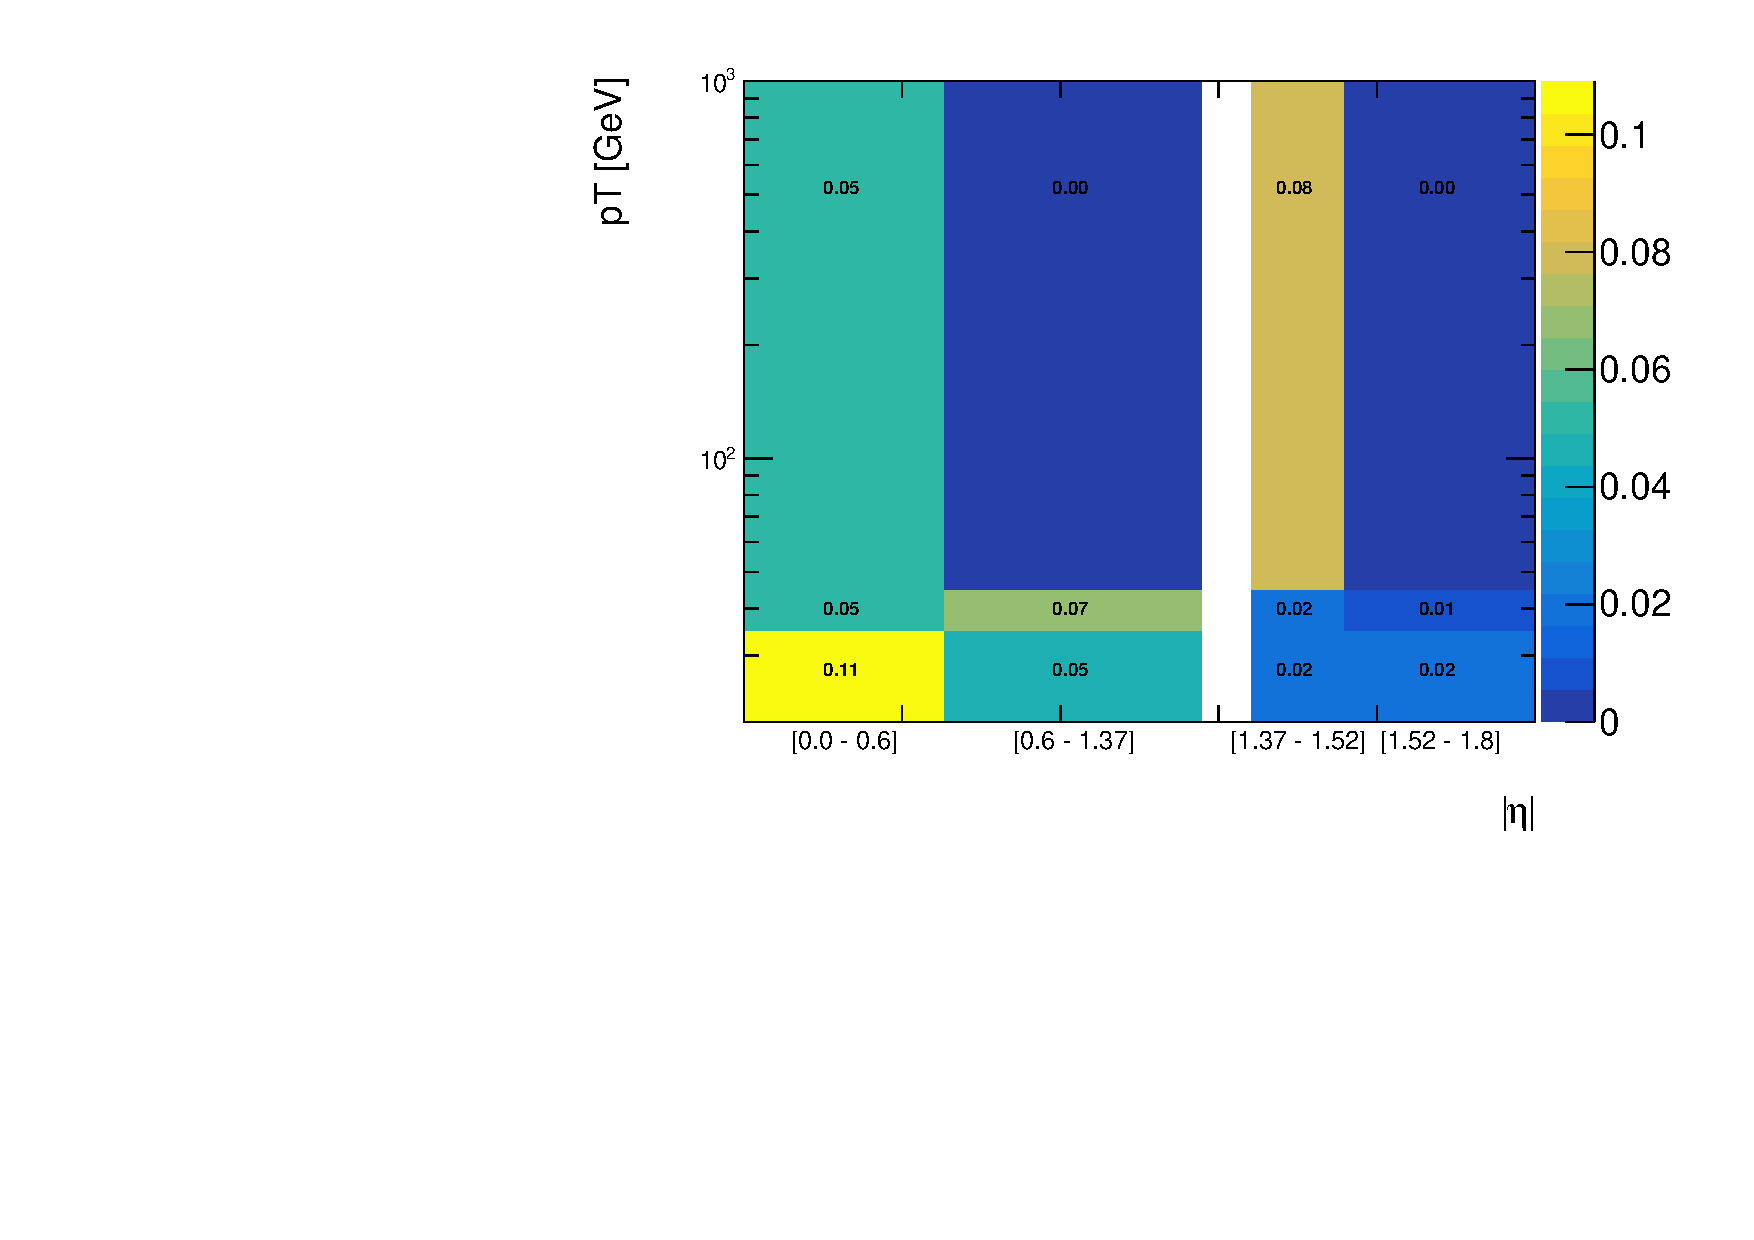
\includegraphics[width=0.45\textwidth]{figures/egammafakes/diffchangingMassWindow.pdf}}

\caption [] {Impact of the sources of systematic uncertainties for the converted photon case. The numbers show the relative uncertainty with respect to the nominal SFs in each bin. The sources of uncertainty are: (a) the signal function is changed to MC template. (b) the background function is varied to Gaussian. (c) variation of the fitting mass window in both sides by 5 GeV.}
%
%{\includegraphics[width=0.45\textwidth]{figures/egammafakesun/converted_ph/Postfit_Zpeak_PtBin1_EtaBin6_zee.pdf}}
%\phantomcaption 
\label{fig:impact_of_uncertainty_converted}
\end{figure}

\newpage

\begin{figure}[!htbp]
\centering
\subfloat[]{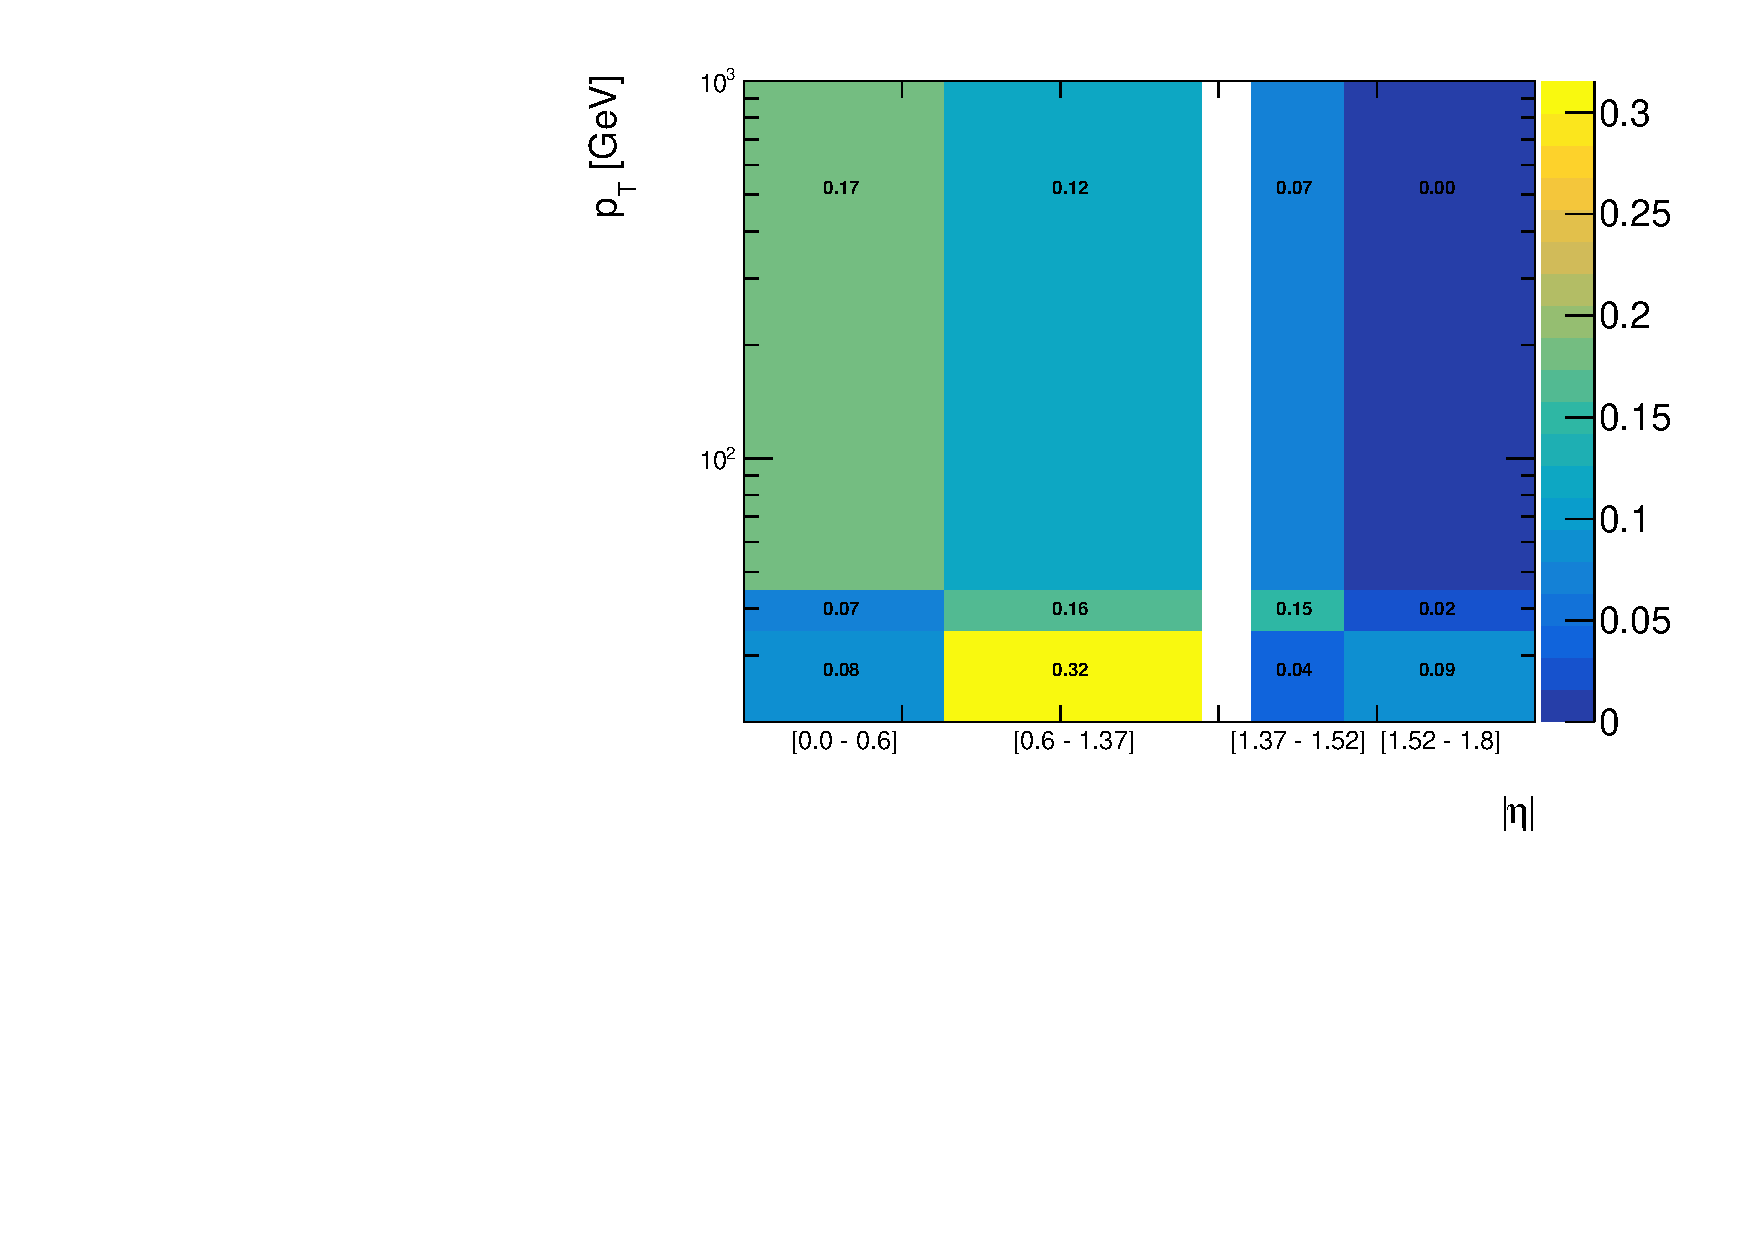
\includegraphics[width=0.45\textwidth]{figures/egammafakes/undiffchangingSigtoMCtemplate.pdf}}
\subfloat[]{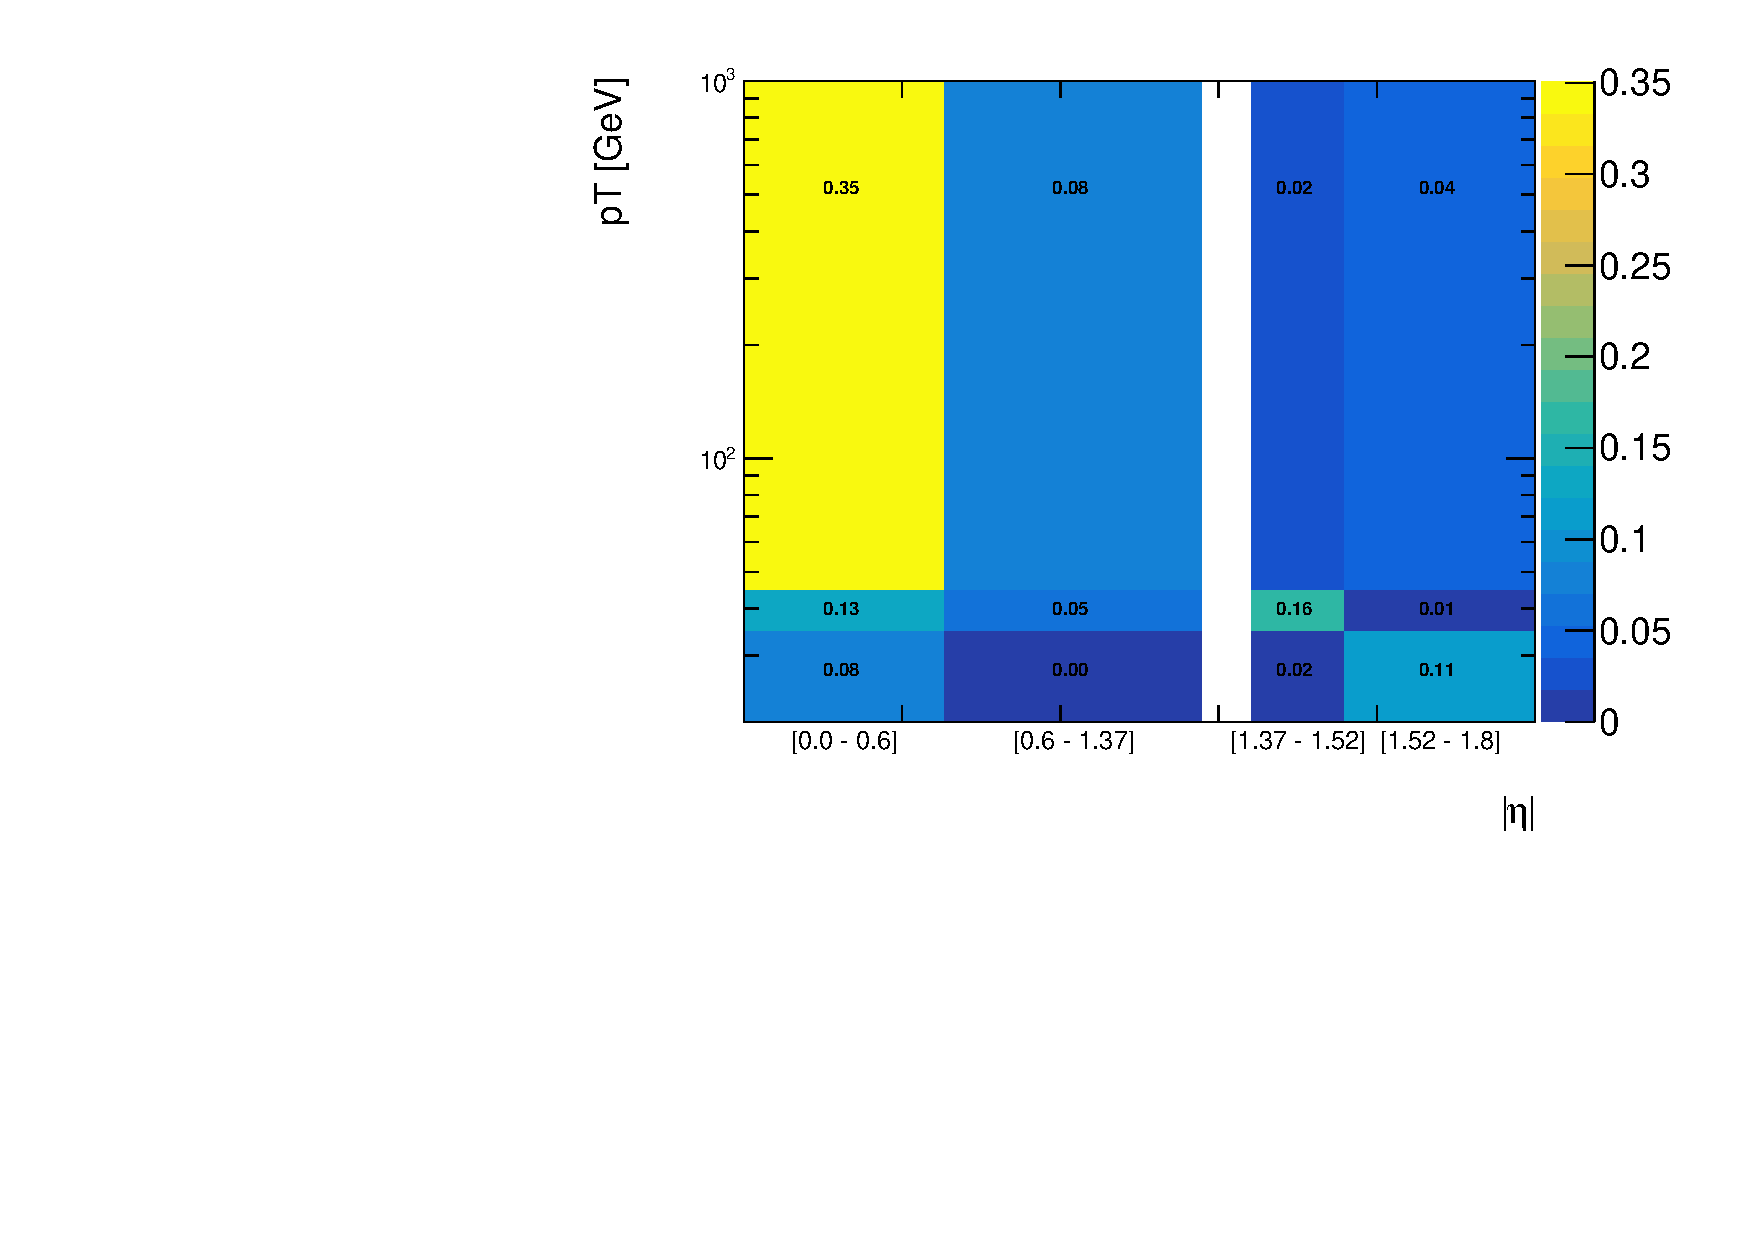
\includegraphics[width=0.45\textwidth]{figures/egammafakes/undiffchangingBkgtoGaus.pdf}}
\quad
\subfloat[]{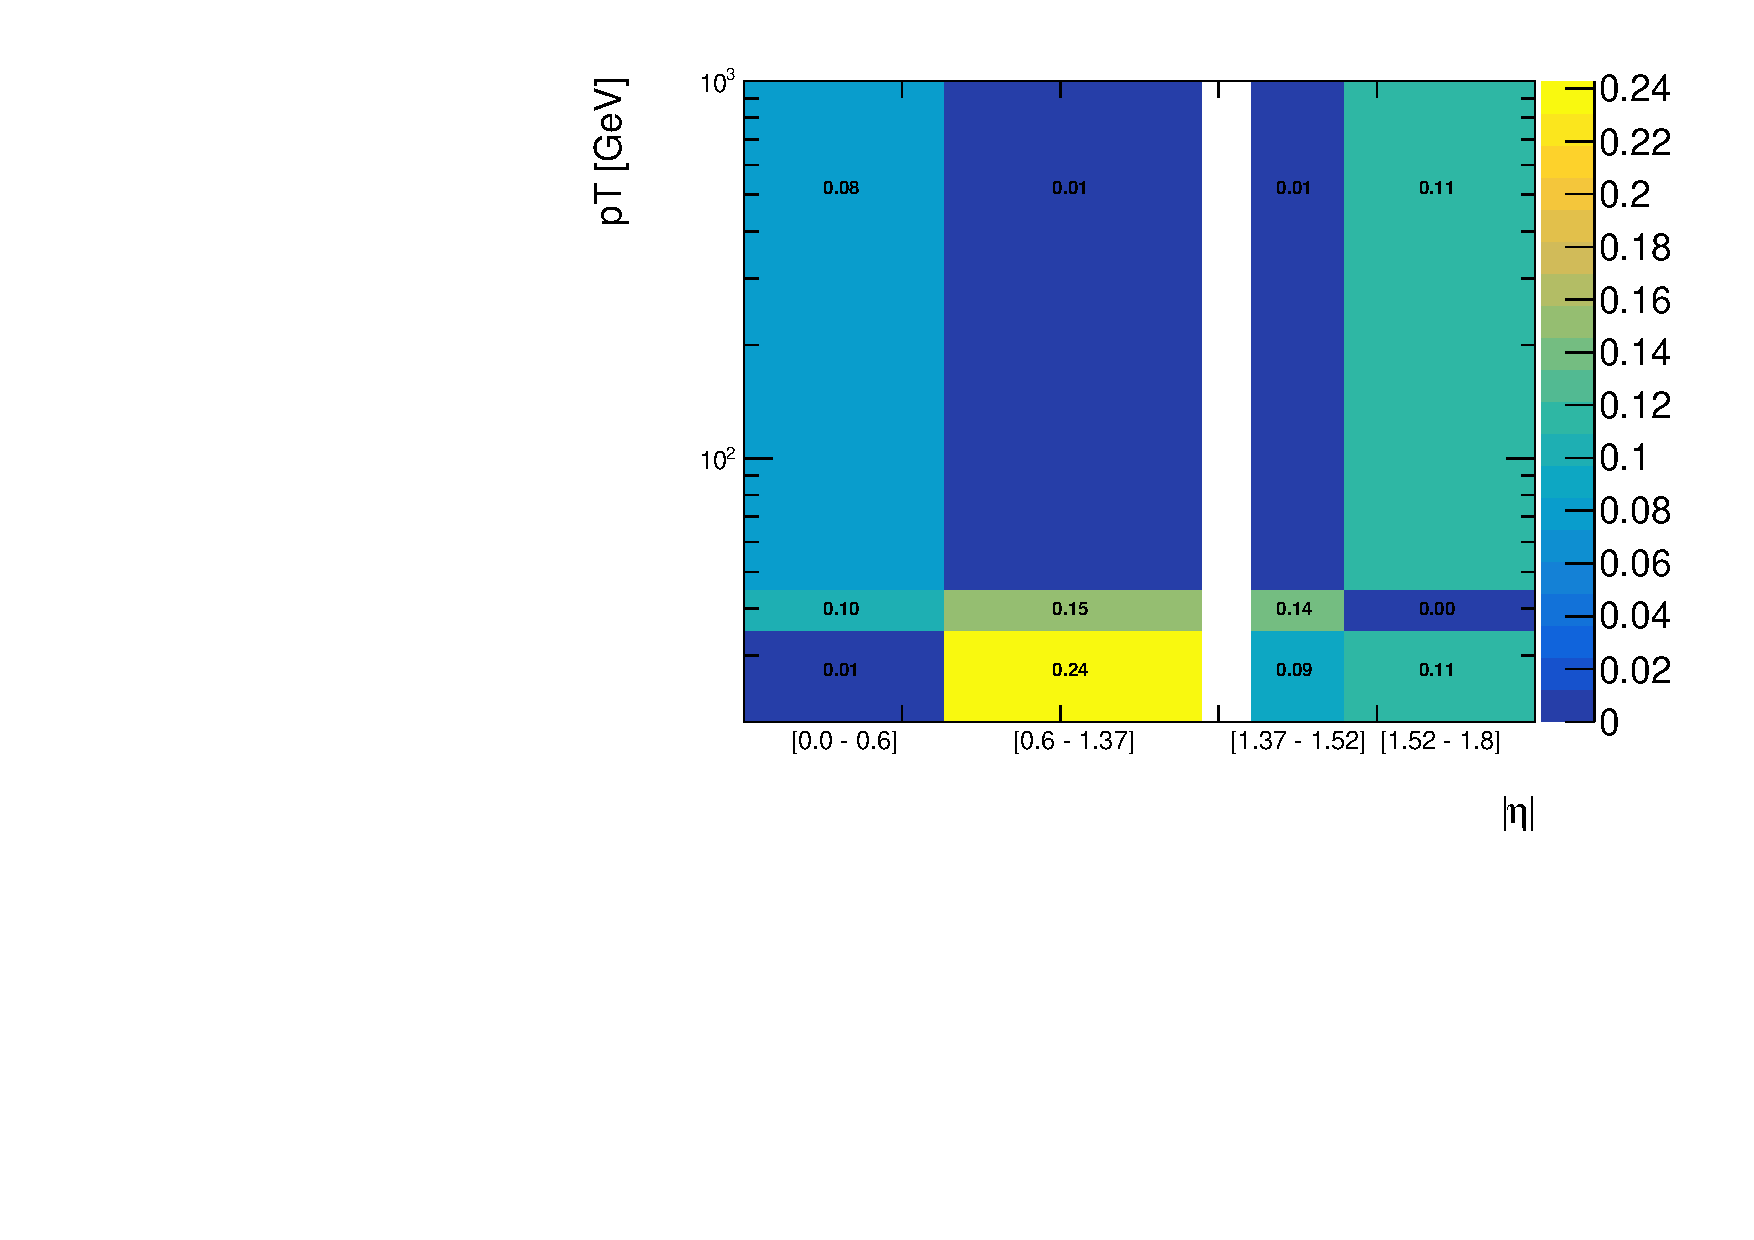
\includegraphics[width=0.45\textwidth]{figures/egammafakes/undiffchangingMassWindow.pdf}}

\caption[] {Impact of the sources of systematic uncertainties for the unconverted photon case. The numbers show the relative uncertainty with respect to the nominal SFs in each bin. The sources of uncertainty are: (a) the signal function is changed to MC template. (b) the background function is varied to Gaussian. (c) variation of the fitting mass window in both sides by 5 GeV.}
%{\includegraphics[width=0.45\textwidth]{figures/egammafakesun/converted_ph/Postfit_Zpeak_PtBin2_EtaBin6_zee.pdf}}
%\phantomcaption 
\label{fig:impact_of_uncertainty_unconverted}
\end{figure}

\FloatBarrier
